\setcounter{chapter}{3} %this gives Chapter 4
\chapter{Apparatus}
\label{chapter:apparatus}

This chapter introduces the experimental setup. First the vacuum system will be described, then the laser system, optical setup, the detection system and the experimental and control electronics.

The complete apparatus was built from scratch. It was designed to address requirements different from those of our research group's previous ion trap experiments. The new apparatus was intended to test a number of different ion trap designs, which involves the replacement of the ion trap (or the whole vacuum system) more frequently. To make this replacement easier, a modular design philosophy was adopted.

Single-mode optical fibres were used to transport light from the lasers to the optics in the immediate vicinity of the trap. This decouples the optical alignment at the input and output side of the fibre. Changes in the alignment that occur in these optical setups, such as creeping with changing temperature or accidental movement of optical elements, cannot propagate through the whole system. If there is a change in alignment on the fibre input side, it results in loss of power on the output side, not misalignment. This provides greater stability and easier maintenance. 

The vacuum system was standardised. The same type of vacuum chamber was used with two new ion traps. This makes the preparation of the system easier, and several devices in the apparatus (most importantly the whole optical detection system) are reusable for a range of different ion traps in the future.


\section{Vacuum system}

\begin{figure}[t]
\centering
\includegraphics[width=8cm]{chapter4/vacuum/vacuum_chamber_scheme4}
\caption[Vacuum chamber schematics]{Vacuum chamber cross section, showing the position of the trap, main detection window, Ca ovens and direction of the photoionisation beam. \cversion}
\label{fig:vacuum}
\end{figure} 

\subsection{Vacuum chamber}

A hemispherical vacuum chamber, manufactured by Kimball Physics, was adopted (see Figure~\ref{fig:vacuum}). Its small size makes it easier to lift it out of the optical system and place it in a bake-out oven. It has good optical access through a number of viewports. The main viewport has 4.5 inch (114 mm) diameter. There are two additional viewports of 2.5 inch (64 mm) on the side of the chamber and a 1.33 inch (34 mm) viewport on the top. Another 1.33 inch opening on the bottom of the chamber was used for attaching vacuum pumps and a gauge, as well as for routing some of the electrical wiring.

\subsection{Sandia trap}
\label{subsec:sandiatrap}

The experiments described in subsequent chapters were conducted using a DTO Module 4 ion trap (referred to in the following as the ``Sandia trap'') provided by Sandia National Laboratories in Albuquerque, New Mexico, USA. It has a planar electrode arrangement on a chip carrier (Figure~\ref{fig:sandiatrap}). 14 DC control electrodes are arranged around a $ 2000\um \times 400\um$ slot cut into the carrier. Along the slot, there are 2 RF rails, approx. 10\um\, wide and 200\um\, apart. The trapping axis is along the slot, in between the RF rails.

The trapping region is centred on a $8\mm \times 8\mm$ high resistivity silicon (HRS) substrate, which has a 1\um\, thick top layer of silicon-oxy-nitrate (SiO$_x$N$_y$). Both the DC and the RF electrodes are made of tungsten  with a complex ring structure, to withstand stress from high electrostatic forces. The DC electrodes have a 0.5\um\, thick aluminium covering layer, but this layer does not extend right to the edge nearest the trapping region, stopping 10\um\, short. The RF rails are connected to their bonding pads via an air bridge, suspended over the substrate. The chip is mounted on a Kryocera pin grid array package. The bottom of the package has a counter-sunk slot for better optical access to the trapping region. The open substrate surface close to the trap and the bottom of the electrodes are gold coated. The coating on the substrate surface reduces charge build-up, which would lead to stray electric fields. On the front face the electrodes have an aluminium coating, while the substrate is bare silica. Newer versions of the same trap design, used by other research groups, have gold coating on the front face of the substrate as well.

\begin{figure}[t]
\begin{center}
$\begin{array}{cc}
\mbox{\bf (a)} & 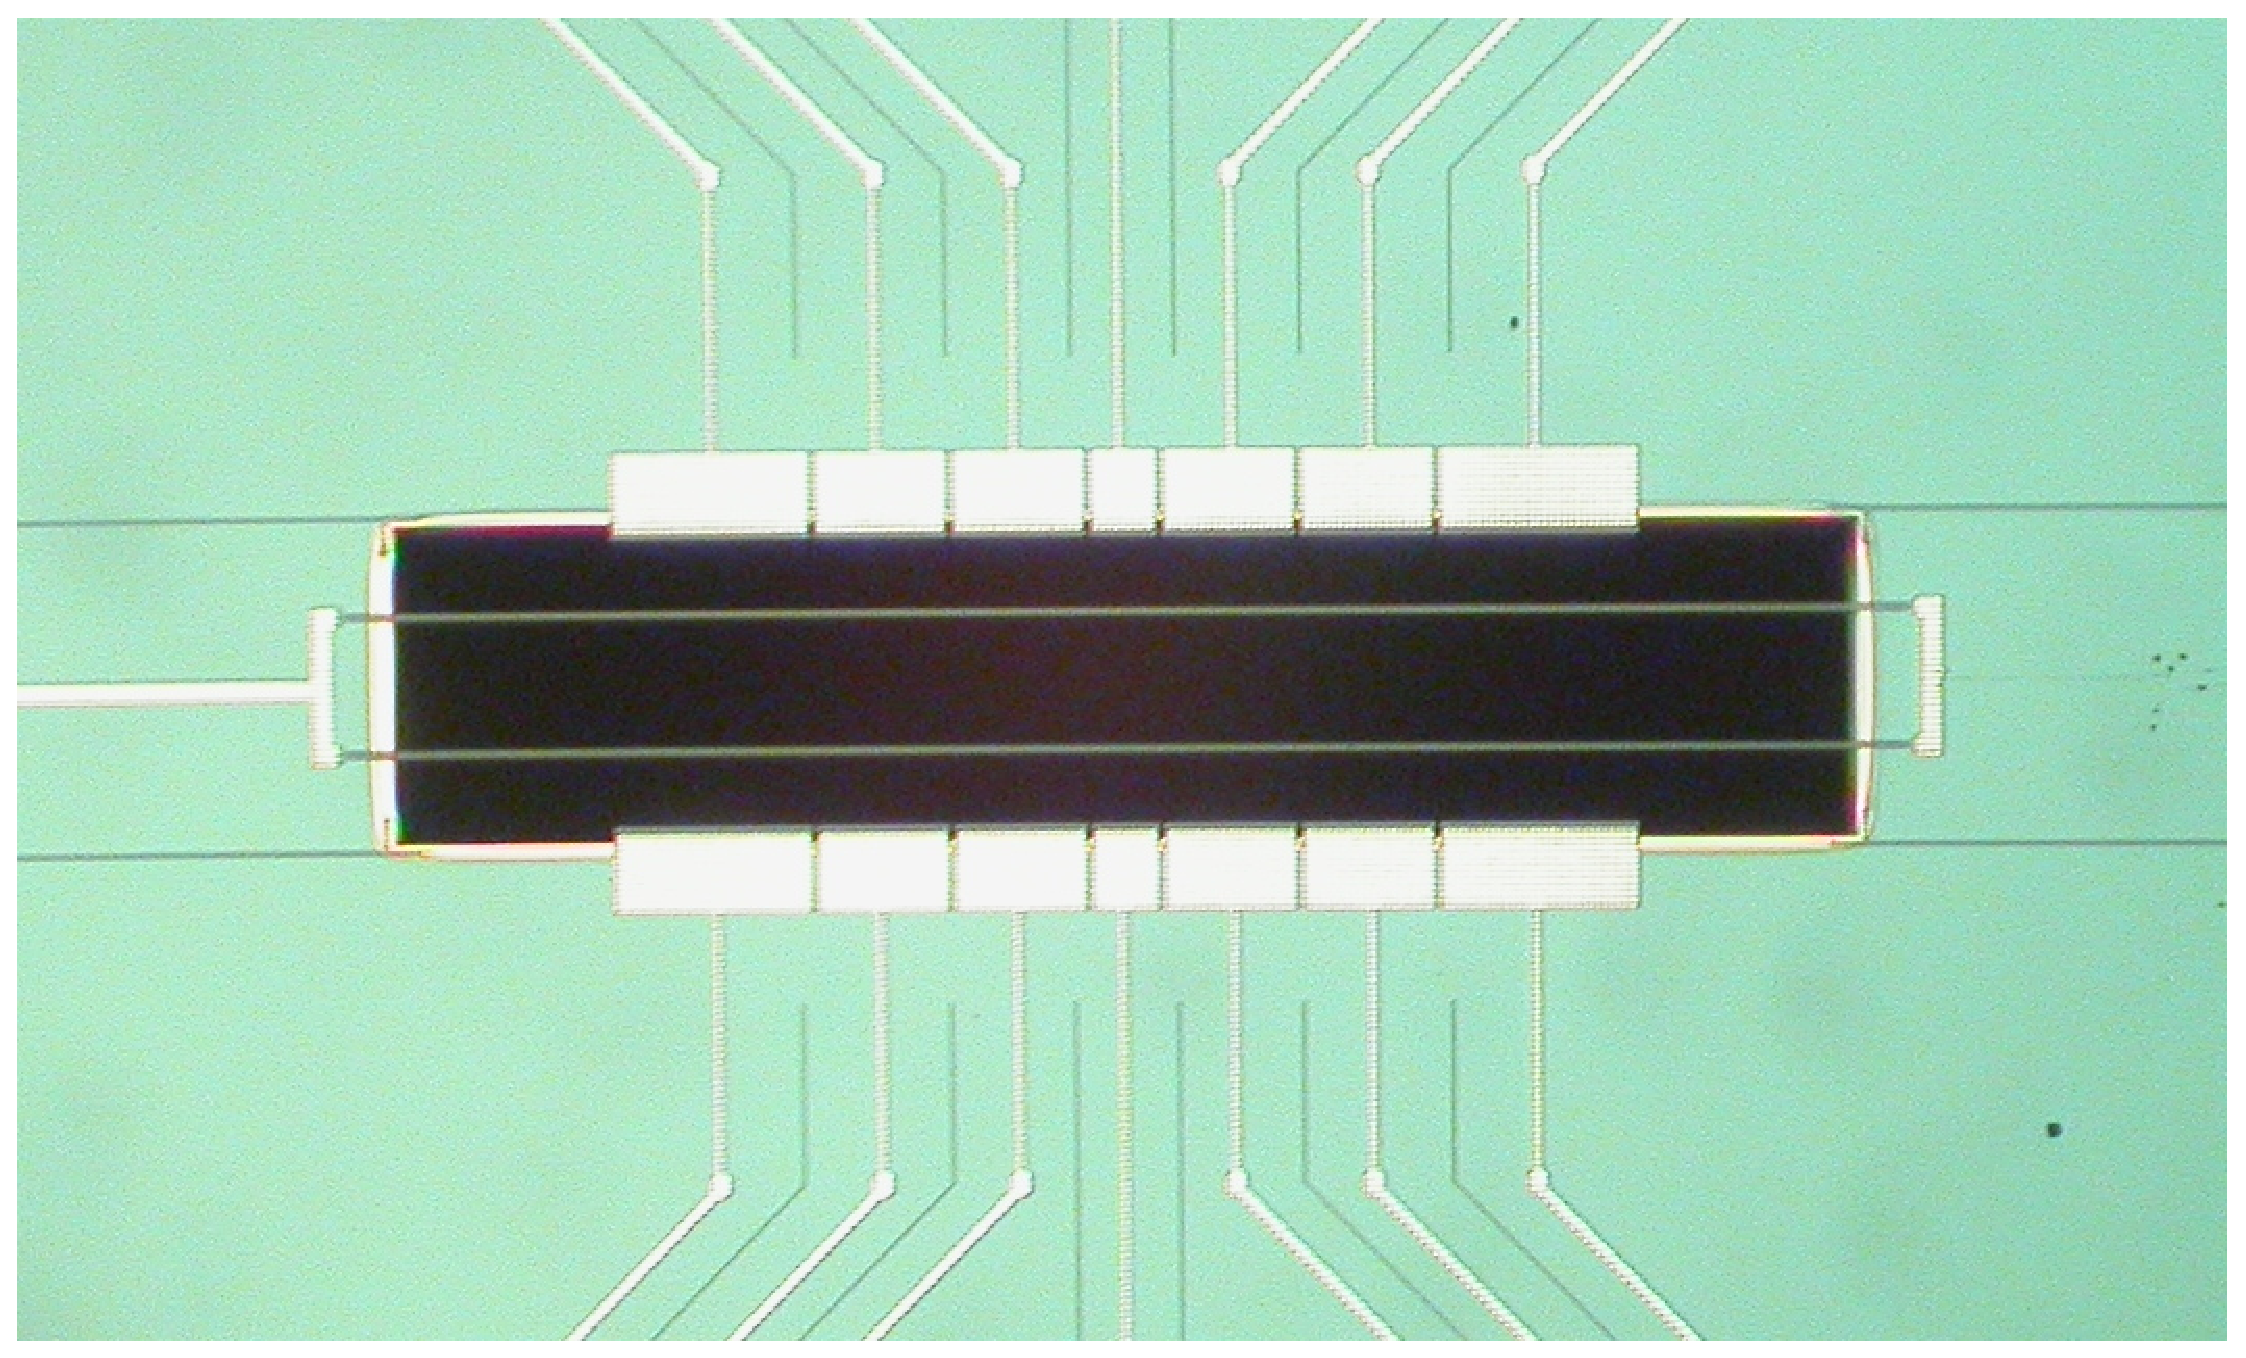
\includegraphics[width=9cm]{chapter4/sandia/trapphoto}\\
\mbox{\bf (b)} & 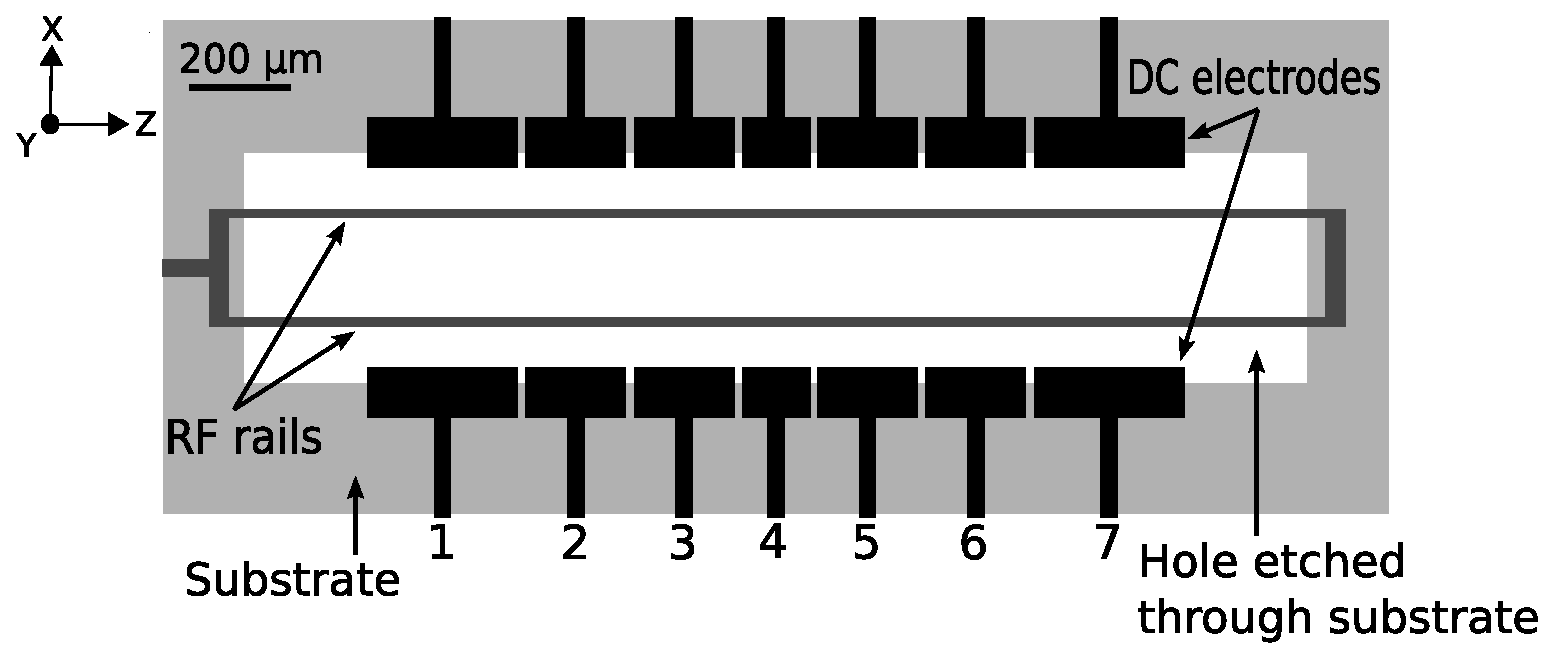
\includegraphics[width=11cm]{chapter4/sandia/trapscheme1d_v3} \\
\end{array}$
\end{center}
\caption[Sandia trap photo and schematics]{a) Photo of the Sandia trap, after removal of the air bridge on the right side, taken with a digital camera through the eyepiece of an optical microscope. b) Schematics of the trap, with the numbering of the electrode pairs (one upper and one lower electrode) for reference. The trapping region is along a line following the middle of the trap, in between the RF rails.}
\label{fig:sandiatrap}
\end{figure} 

% \begin{figure}[h!t]
% \begin{center}
% 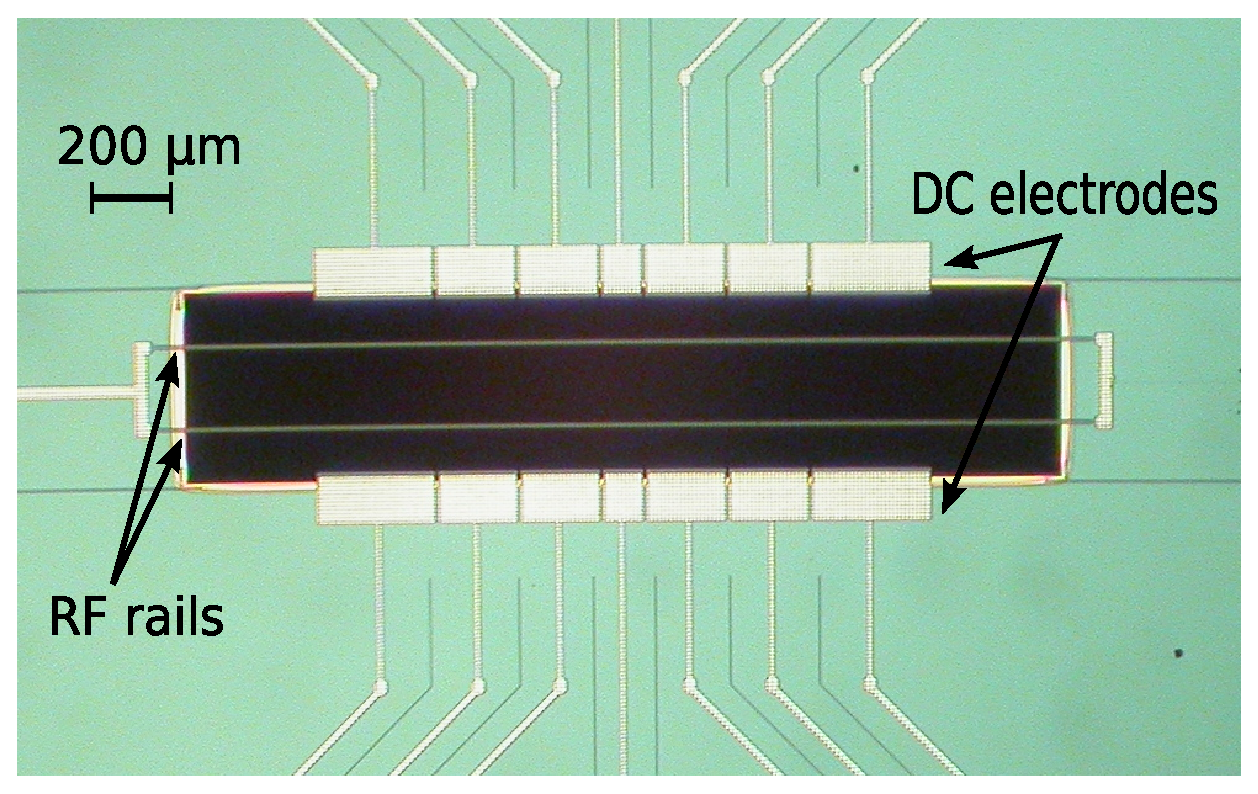
\includegraphics[width=10cm]{chapter4/sandia/trapscheme2}
% \end{center}
% \caption[Sandia trap]{Photo of the Sandia trap, after right airbridge removal, taken with digital camera through the eyepiece of an optical microscope. The trapping region is along a line the middle of the trap, in between the RF rails.}
% \label{sandiatrap}
% \end{figure} 


In the original design of the Sandia trap the RF rails were driven from both ends, to minimise the variation of the RF field along the trap axis. In early testing, however, it was discovered that this arrangement was problematic. When driven from both ends, a small difference in the RF phase at the two ends is hard to avoid. It results in currents flowing in the RF electrodes, and thus ohmic heating. The NIST Ion Trap Group observed heating resulting in a visible white glow of the RF rails, and their subsequent mechanical failure, when driven from both ends.

To eliminate such heating in our trap, the air bridge connection was removed on one side, so that the RF rails are driven from a single voltage source. The air bridge was severed as close to the trap as possible. This is to reduce the excess capacitance between the remains of the removed RF supply line and the front face of the chip (see Figure~\ref{fig:sandiatrap}).

Due to the planar arrangement of the Sandia trap, one has less control over the electric field perpendicular to the trap plane, compared to the in-plane field. An extra electrode wire was therefore attached to the bottom of the chip carrier (a ``compensation electrode''). The electrode is a segment of 0.25mm diameter gold wire connecting two pins on the back of the chip socket. In the middle, the wire was twisted into a spike pointing towards the trapping region. It is connected to the unused pin and the common ground of the Ca oven feedthrough (see Figure~\ref{fig:calciumoven}). The details of the air bridge removal and the compensation electrode are given in \cite{Curtis2007}.

Commercially available chip sockets were incompatible with our UHV requirements. They had high outgassing rates and could not withstand the 200\degC\, temperature that was used in the bake-out of the vacuum system. Custom chip sockets were made, based on a design by the University of Michigan, to mount the Sandia trap, using Vespel, a high performance plastic suitable for UHV operation. 

\subsection{Calcium oven}
\label{subsec:oven}

For a source of calcium, two calcium ovens were installed in the vacuum chamber. Each oven is a thin-walled stainless steel tube with 14\mm\, length and 3\mm\, diameter. Calcium was placed in the tubes by cutting narrow strips from a calcium foil using a clean steel knife, and dropping them into the tubes. One oven contained calcium with its natural isotopic abundance  and the other contained a sample enriched in \CaI{43}. The ends of the tubes were closed by crimping. The oven orifice is a small hole of area 0.3\mm$^2$ drilled in the middle of the tube. The ovens were spot-welded on stainless steel rods (see Figure~\ref{fig:calciumoven}) such that they have one rod each as current input connection and a third rod is their common return. Resistive heating was used to operate the ovens, by passing current (up to 7 A) through them. The feedthroughs and thick steel rods have negligible resistance compared to the thin-walled ovens. See Section \ref{sec:oventest} for further information about the ovens.


\begin{figure}[t]
\centering
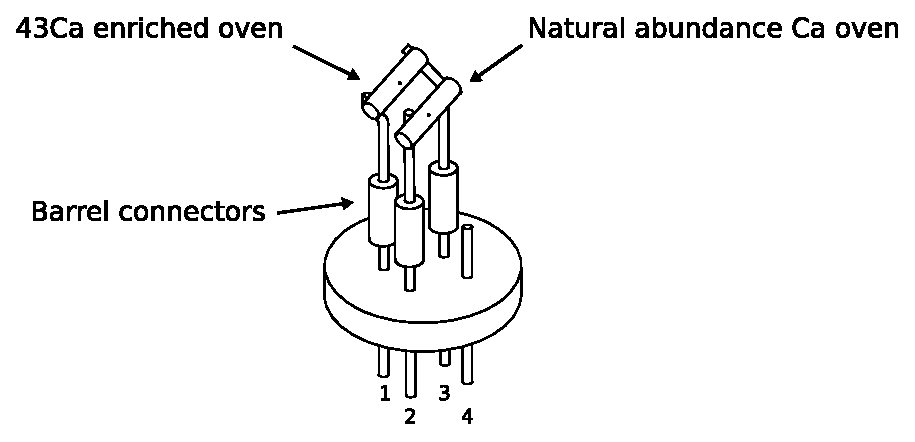
\includegraphics[width=12cm]{chapter4/oven/oven_scheme3}
\caption[Calcium oven schematics]{Schematic view of the feedthrough connected to the Ca ovens. Of the four numbered pins of the feedthrough, (1) is connected to the \CaI{43} enriched oven, (2) is connected to the natural abundance \CaI{} oven, (3) is the common return and (4) is connected to the manually added compensation electrode (see Section~\ref{subsec:sandiatrap}, connection not shown on the figure). Figure based on CAD design of M. Curtis.}
\label{fig:calciumoven}
\end{figure} 

\subsection{Vacuum pumps}

For continuous ultra-high vacuum (UHV) operation of the trap, there are two vacuum pumps attached to the chamber.

The main pump is a Varian VacIon Plus 20 ion pump, which is aided by a SAES SORB-AC GP50 chemical getter pump. The chemical getter pump's role is similar to a titanium sublimation pump: it has higher efficiency in pumping hydrogen, which supplements the capabilities of the ion pump. The chemical getter does not require an external power supply once it has been activated. It is advantageous in vacuum systems which are opened up to air very rarely since its sponge-like structure absorbs gases very quickly and it can be outgassed only very slowly, and in systems where having a hot filament (as in the titanium sublimation pump) is not feasible. In our system, however, the pump is well separated from the main vacuum chamber, so having a hot filament is not a problem, and opening up the vacuum to carry out repairs and changes of equipment is not uncommon. In future the chemical getter pump is therefore likely to be replaced with a titanium sublimation pump.

The pressure is measured on a Varian UHV-24 ion gauge, with reliable pressure measurements down to  $5 \times 10^{-11}$\torr\, and reduced performance down to $5 \times 10^{-12}$\torr.


\section{Optical setup}

To trap and cool ions, four laser frequencies are needed. These are: 423\nm\, and 389\nm\, light for neutral atom excitation and photoionisation respectively, 397\nm\, and 866\nm\, light for Doppler cooling and repumping (see Figure~\ref{fig:levels}). Additionally a 854\nm\, laser was set up later in the experiment, to prevent shelving in the 3d~$^2$\dfh\, level.


The two photoionisation lasers were shared between different experiments. Beams were brought to the trap via an optical fibre from another laboratory room. The optical setup at the fibre input end  is described in section \ref{subsec:photionlayout}.

The other three lasers were placed on a separate optical table from the vacuum system. Their layout was designed to fit the available space. A modular approach was adopted, meaning that the basic layout is common for all the systems, while it still allows for differences arising from the different requirements posed on the lasers. This makes possible relatively quick deployment of an additional laser system if needed.

In the common part of the design the laser beam goes through an optical isolator and is reflected from a diffraction grating. The grating's role is to create three separate beams (using orders -1, 0 and +1), and act as a coarse filter to clean up the spectrum. Order -1 is used for the ``experimental beam'', eventually coupling into a fibre which is connected to the trap optical setup. This order is arranged to have the highest power. Orders 0 and +1 respectively are used to lock the laser frequency to an external cavity and for frequency diagnostics.

Our lasers are of the Toptica DL100 series, with various laser diodes. Inside the laser's casing, the system is arranged in Littrow configuration, in which a grating provides optical feedback to the laser diode. This results in stable single-mode operation and narrower linewidth.

The following sections provide details of the individual laser systems. 


\subsection{866nm repumping laser setup}
\label{subsec:866setup}


\begin{figure}[h!t]
\centering
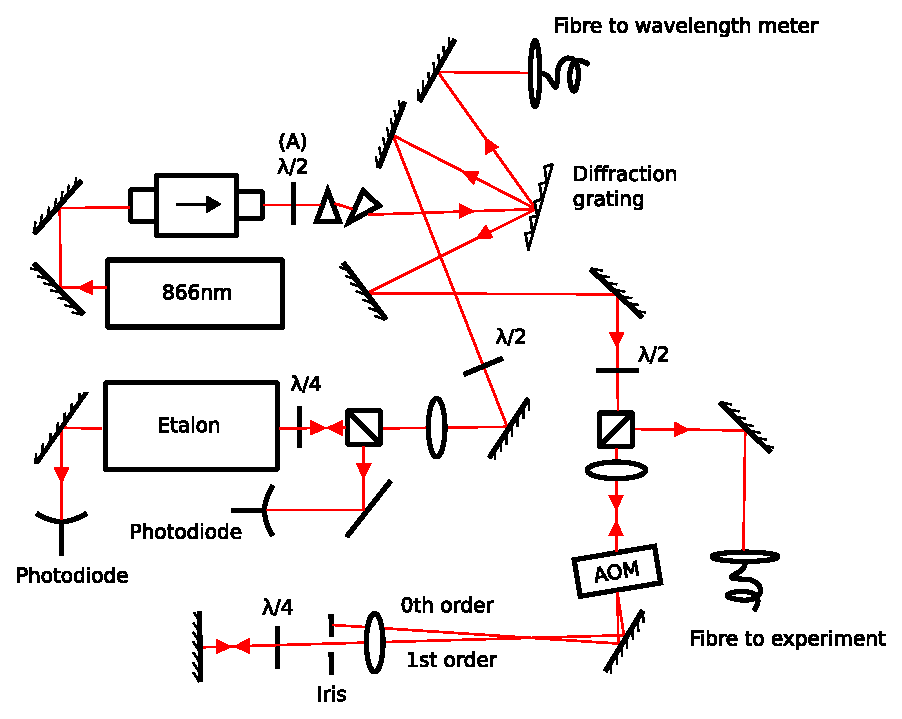
\includegraphics[width=13cm]{chapter4/866layout/866layout_v3}
%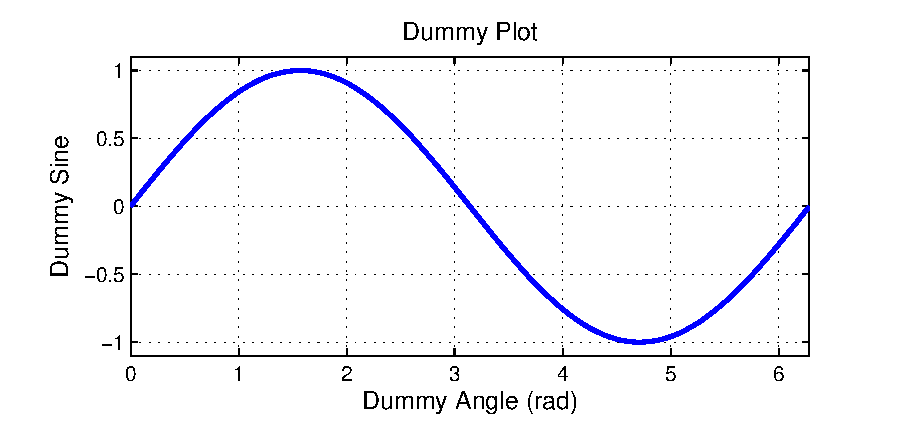
\includegraphics[width=5cm]{dummy}
\caption[866nm laser layout]{Layout of the 866nm laser system. Details in the text. Arrows on the beampaths show the direction of beam propagation. (Colour in electronic version)}
\label{fig:866layout}
\end{figure} 

% \begin{figure}[h!t]
% \centering
% %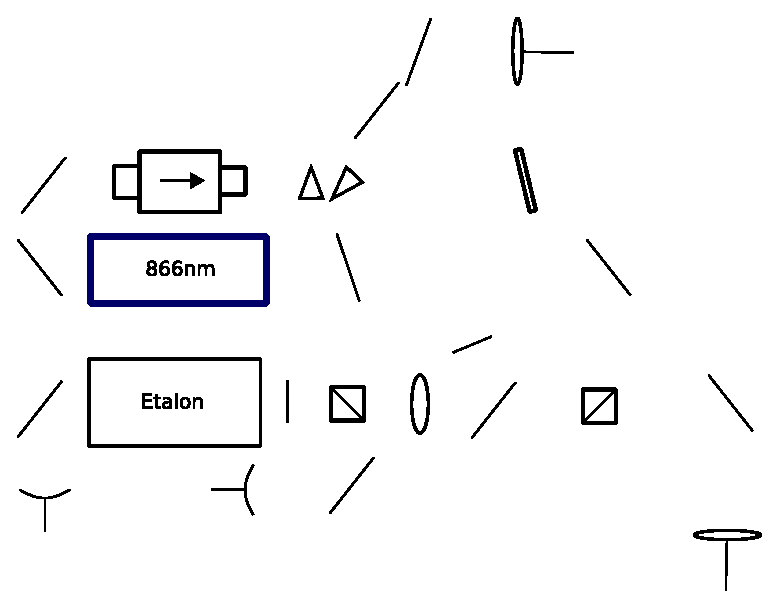
\includegraphics[width=10cm]{chapter4/866layout/866layout_v1}
% 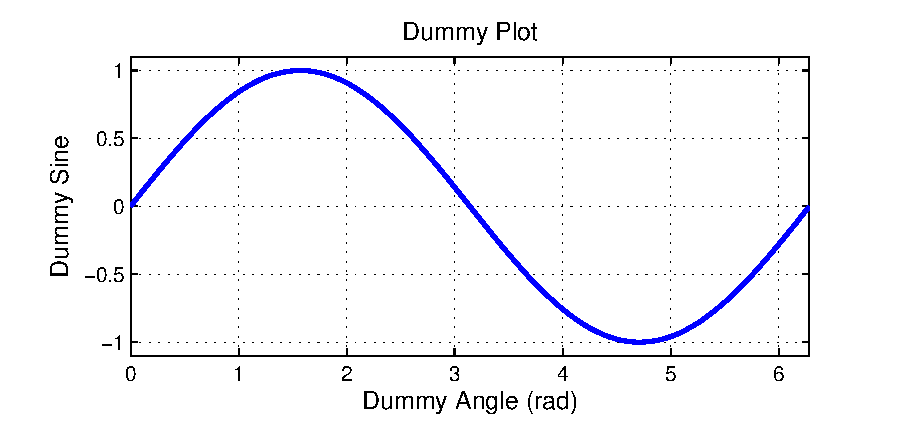
\includegraphics[width=5cm]{dummy}
% \caption{Beam profiles}
% \label{866beamprofile}
% \end{figure} 


\begin{figure}[h!t]
\begin{center}
$\begin{array}{c}
\mbox{\bf (a)} 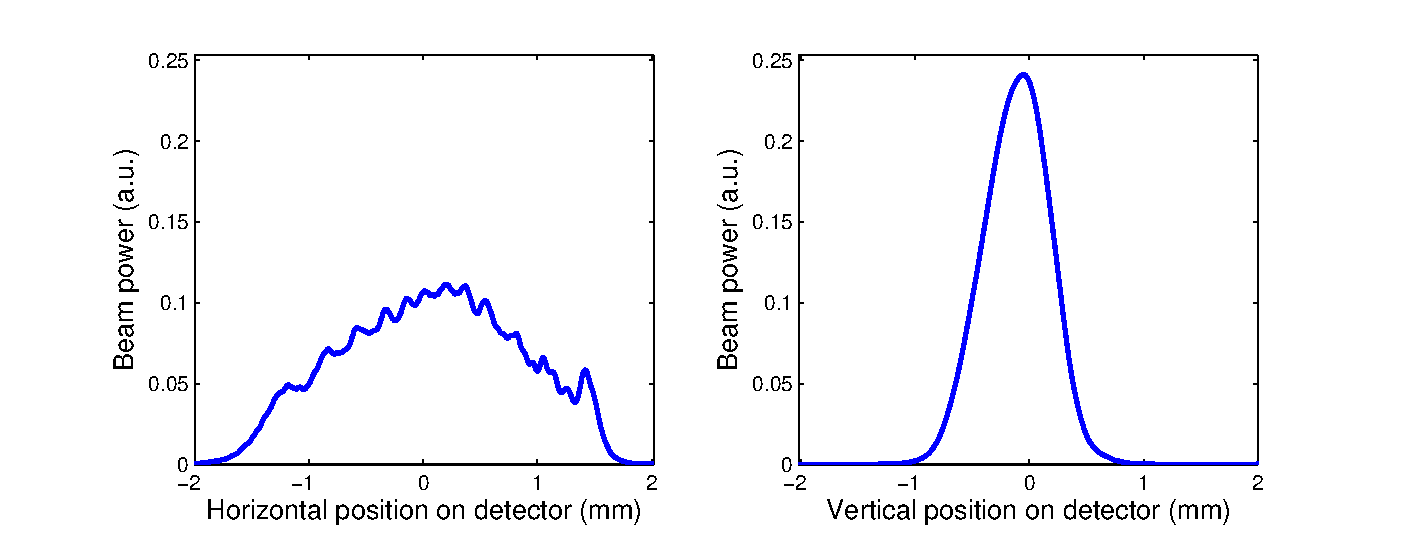
\includegraphics[width=13cm]{chapter4/beamprofile/866_laser_out}\\
\mbox{\bf (b)} 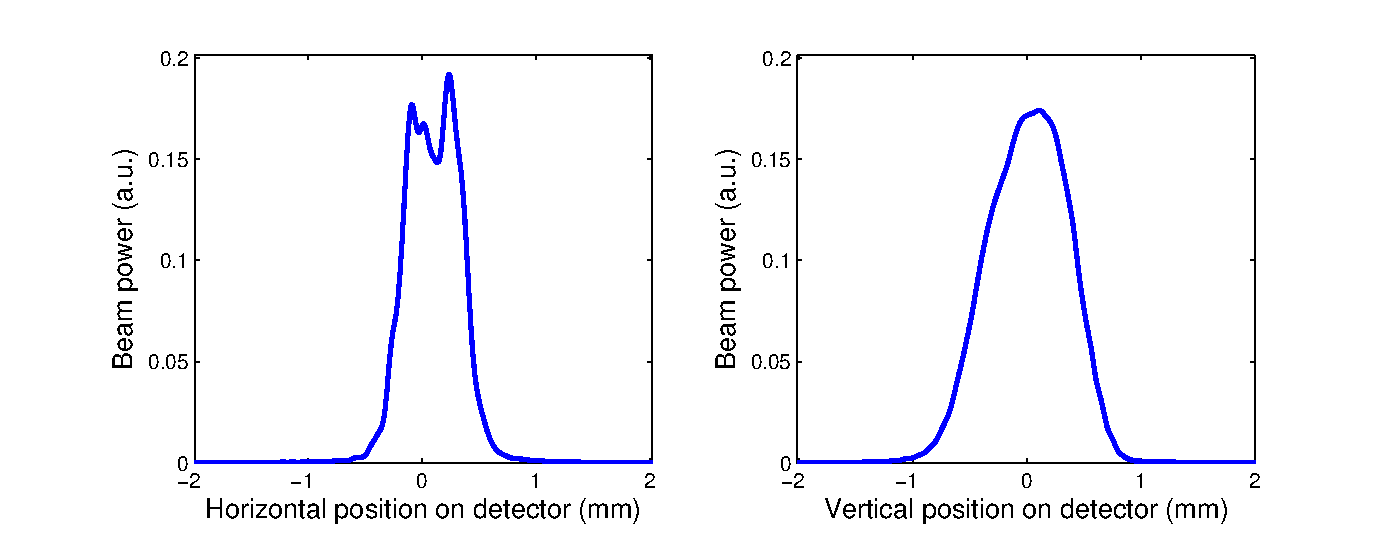
\includegraphics[width=13cm]{chapter4/beamprofile/866_after_prism_pair}\\
\mbox{\bf (c)} 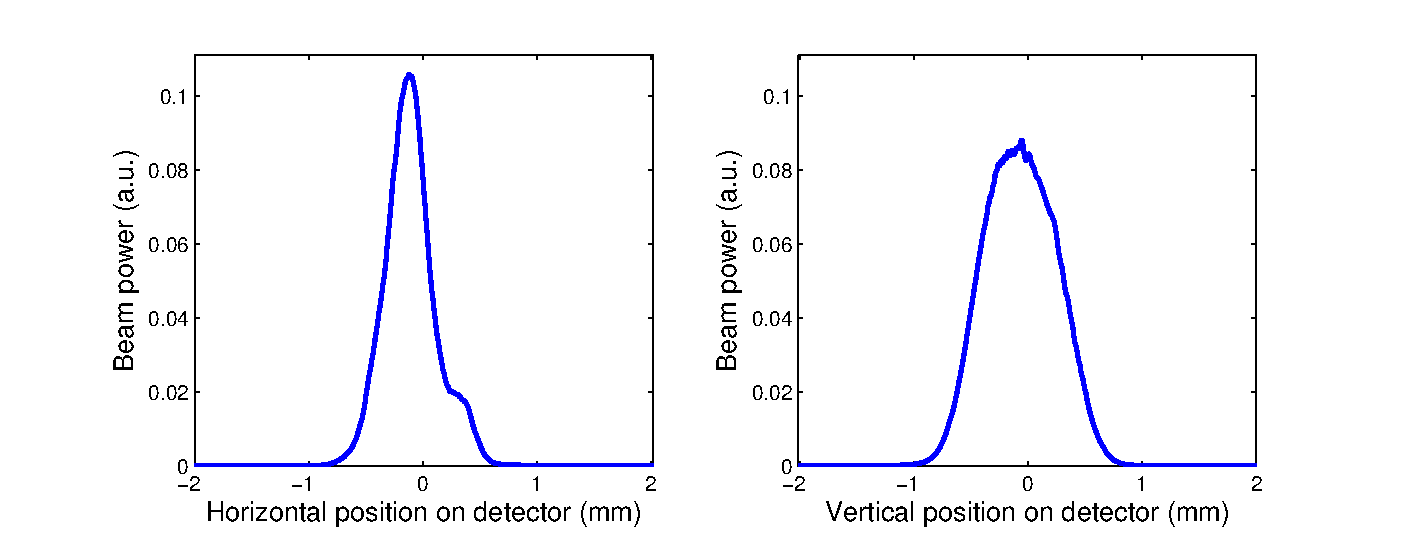
\includegraphics[width=13cm]{chapter4/beamprofile/866_before_fibre_in}\\
\end{array}$
\end{center}
\caption[Beam profiles of the 866nm laser]{Beam profiles of the 866nm laser, at different points in the optical path (obtained with Thorlabs BP104-UV beam profiler). a) the laser output, b) after an anamorphic prism pair, c) the ``experimental beam'' before its fibre input. Laser intensities are in arbitrary units. The laser output is elongated horizontally, a disparity which is reduced by the prism pair. The ``wiggles'' visible on the top left and middle left profiles are generally caused by Fresnel diffraction, because of optical cut off at the focusing lens on the laser diode.}
\label{fig:866beamprofile}
\end{figure}


The main requirement of the 866\nm\, laser is high output power, at least of the order of 1\mW\, at the ion. The optical layout is shown in Figure~\ref{fig:866layout}.

The output of the laser box is guided through an optical isolator to reduce optical feedback. A $\lambda/2$ waveplate (A) sets the optimal polarisation for an anamorphic prism pair, which is used for beam shaping. Beam shaping is necessary to create a more circular beam as the diode laser output is generally highly elliptical (see Figure~\ref{fig:866beamprofile}). The prism pair greatly improves the performance of the later optical elements, especially the coupling efficiency into fibres.

It is also possible to rotate the $\lambda/2$  waveplate (A), in order to change the proportions of laser power of the beams after the diffraction grating. Thus, if needed, more power can be diverted into the locking circuit and to the wavelength measurement, at the expense of power going to the experiment.

A Newport 53-004ZD02-035R diffraction grating (gold coating, 830 grooves/mm, blaze wavelength of 900nm) was used to divide the beam into three beam paths as explained above. Order +1 (the topmost reflected beam in Figure~\ref{fig:866layout}) is coupled into a multimode fibre, which leads to the wavemeter for frequency measurements. This grating performs a significant ``cleaning up'' role on the spectral composition of the experimental beam, eliminating wide wings (up to several \nm) associated with amplified spontaneous emission in the laser diode.

\subsubsection{Frequency stabilisation of the 866nm laser}
Order 0 is used for frequency stabilisation with an external cavity. In the beampath a $\lambda/2$ waveplate sets the polarisation to maximise the transmission of a polarising beam splitter (PBS) cube, and a 250mm  focal length lens focuses the beam to the centre of the NPL reference cavity. At this point of the layout, given the available equipment, we had two possibilities for stabilising the laser frequency: side-of-fringe lock or Pound-Drever-Hall (PDH) locking.

%One can use a photodiode to monitor the cavity transmission, and lock to the side slope of the transmission profile (side-of-fringe lock). This is simpler to implement, though has smaller capture range and generally provides a less stable laser frequency than the PDH lock. 

The former is much simpler to implement. One uses a photodiode to monitor the cavity transmission and locks to the side slope of the transmission profile. With the PDH method one monitors the cavity reflection with a high speed photodiode when the laser frequency is modulated. The photodiode output is demodulated and provide the error signal. This arrangement gives better frequency stability than side of fringe locking, with improved capture range (twice the modulation frequency of the laser). A detailed description is given  in Chapter 5 of the PhD thesis of B. Keitch \cite{Keitch2007} and in \cite{Drever1983}. 

% \begin{figure}[h!t]
% \centering
% 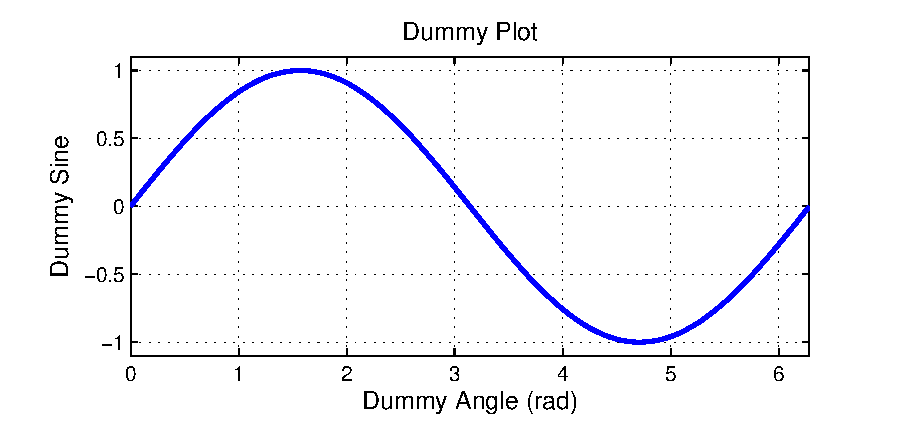
\includegraphics[width=5cm]{dummy}
% \caption[Locking signal]{Locking signal: side-of-fringe, PDH}
% \label{locksignal}
% \end{figure} 

Because of these advantages over the side-of-fringe lock, the PDH arrangement was first implemented. The laser frequency was modulated by modulating the current of the laser diode. This was done by the KILL control module built by B. Keitch, which supplies the appropriate RF frequency, and also demodulates this frequency from the detection photodiode signal. The demodulated signal is then used by the Toptica locking module to stabilise the laser frequency. The modulation frequency in our case was 170 MHz. This results in sidebands appearing next to the carrier optical frequency, with separation equal to the modulation frequency. The sidebands, however, introduced difficulties in conducting and interpreting the experiments, as it makes the frequency spectrum more complicated, with the appearance of many peaks and dark resonances. This effect can be eliminated by modulating the laser frequency not with the diode current directly, but using an electro-optical modulator (EOM) in the locking beam path, which introduces sidebands for that beam only. That is the approach that we adopted in the case of the 397nm laser (see next section). Alternatively, one can use a different locking mechanism. Because of the ease of setup of the side-of-fringe lock and the already good stability of the 866nm laser (even unlocked) we opted to use side-of-fringe lock for most of our experiments.

The frequency tuning of the laser is done by changing the length of the locking cavity by applying a voltage to the piezo crystal that holds one of the mirrors of the cavity. The voltage on the piezo crystal was set by a DC piezo driver, and this voltage was fine-adjusted by the experimental control computer. The frequency calibration as a function of this control voltage was experimentally determined. The calibration depends on the base voltage of the piezo driver, and it is non-linear over long ranges. 

The control voltage produced by the experimental control computer was adjusted along its whole range [-2.5\V, +2.\V], and the frequency was read off from the wavelength meter. The explored frequency region was small enough that the calibration can be approximated with a linear function. The recorded calibration data is plotted in Figure~\ref{fig:lasercalib} and the fitted voltage dependence of the laser frequency is shown in Table~\ref{tab:lasercalib} on page~\pageref{tab:lasercalib}. The base voltage of the piezo driver is also shown, since the calibration is valid only using similar base voltages, due to the non-linear response of the piezo crystal.

\begin{table}[h!t] 
\centering % used for centering table 
\begin{tabular}{|c||c|c|c|} % centered columns (4 columns) 
\hline                        %inserts double horizontal lines 
Laser & Piezo base (\V) & Calibration (\MHz/\mV) & Resolved freq. steps (\MHz)\\
%heading 
\hline
397\nm & 41 & 0.211(6) & 0.52 \\
% \hline % inserts single horizontal line 
866\nm & 54.3 & 1.77(6) & 4.3 \\
[1ex] % [1ex] adds vertical space 
\hline %inserts single line 
\end{tabular} 
\caption{Calibration information of the Doppler-cooling and repumping lasers (as of 16.7.2007). The resolved frequency steps are due to the 12-bit resolution of the controlling DAC.}
\label{tab:lasercalib} % is used to refer this table in the text 
\end{table} 


%\begin{figure}[h!t]
%\begin{center}
%$\begin{array}{cc}
%\mbox{\bf (a)} 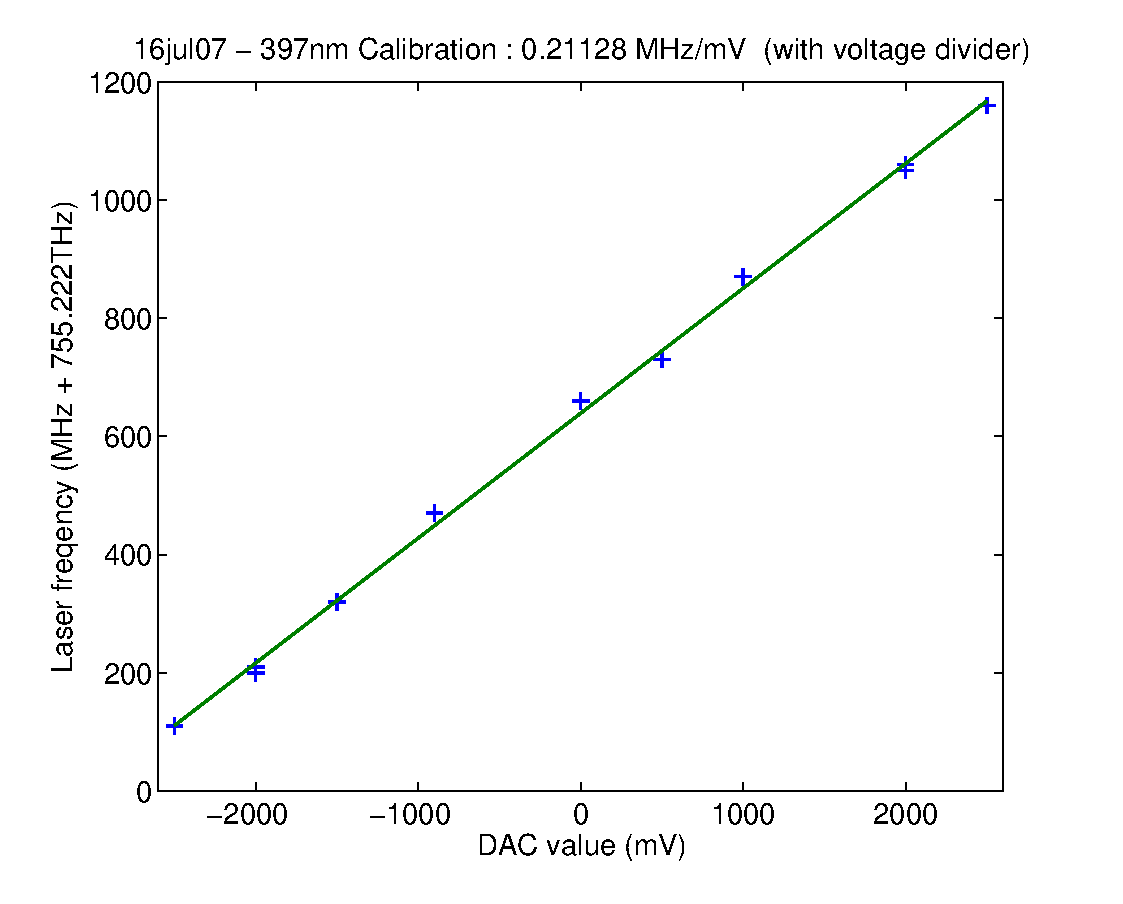
\includegraphics[width=7cm]{chapter4/calib/397calib} &
%\mbox{\bf (b)} 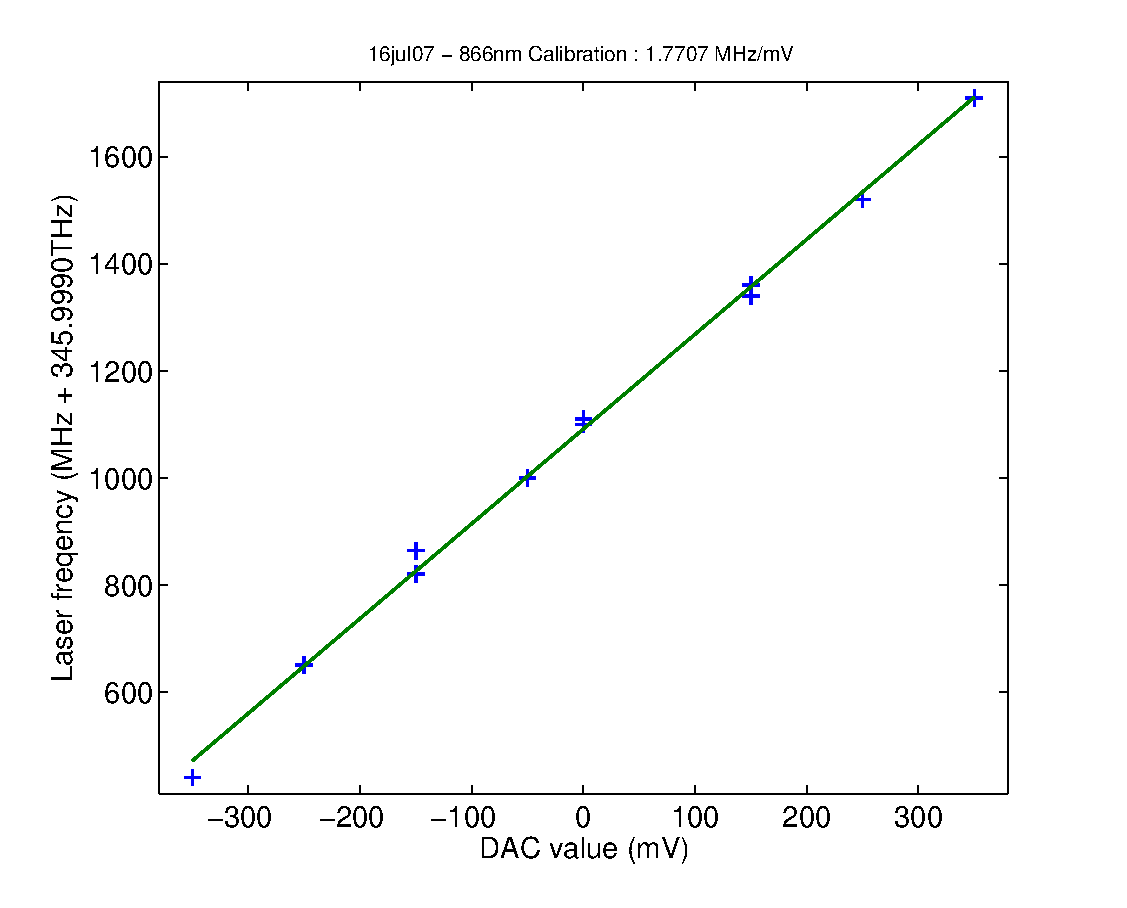
\includegraphics[width=7cm]{chapter4/calib/866calib} 
%\end{array}$
%\end{center}
%\caption[Frequency scanning calibration]{Frequency scan calibration of the 397\nm\, and 866\nm\, lasers. The experimental control computer's DAC output controlled a piezo driver to scan the locking cavity of the lasers. The laser frequencies as measured by a HighFinesse WS/7 Wavelength Meter are shown as a function of the DAC control voltage. The solid lines are linear fits to the data. The slope is shown in Table~\ref{tab:lasercalib}}
%\label{fig:lasercalib}
%\end{figure}

\begin{figure}[h!t]
\begin{center}
$\begin{array}{cc}
\mbox{\bf (a)} 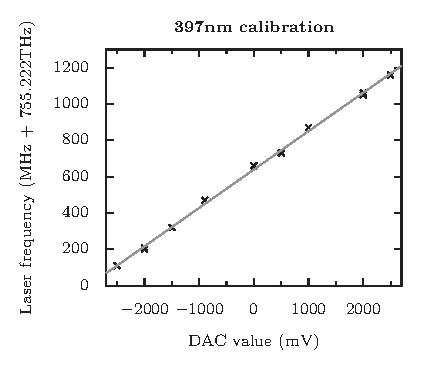
\includegraphics{chapter4/calib/dcalib397_v1} &
\mbox{\bf (b)} 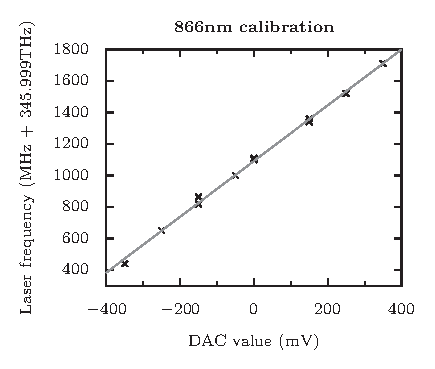
\includegraphics{chapter4/calib/dcalib866_v1} 
\end{array}$
\end{center}
\caption[Frequency scanning calibration]{Frequency scan calibration of the 397\nm\, and 866\nm\, lasers. The experimental control computer's DAC output controlled a piezo driver to scan the locking cavity of the lasers. The laser frequencies as measured by a HighFinesse WS/7 Wavelength Meter are shown as a function of the DAC control voltage. The solid lines are linear fits to the data, the fitted calibration is given in Table~\ref{tab:lasercalib}.}
\label{fig:lasercalib}
\end{figure}


\subsubsection{Experimental beam of the 866nm laser}

Order -1 is used for the experimental beam. To be able to electronically switch the beam on and off, it is guided through a double pass AOM (IntraAction ATM-851A2). The arrangement has approx. $60\%$ double pass maximum efficiency (output power compared to input power when the AOM is on), and extinction of the order of $10^{-6}$ (residual intensity when the AOM is turned off). 

The output beam is picked off with a PBS cube, and coupled into a single-mode, polarisation maintaining (PM) fibre (Nufern PM780-HP) with a Sch\"{a}fter and Kirchhoff 60SMS coupler. The fibre has angle-polished faces (APC) to reduce back reflection and an angled fibre arrangement inside the coupler to increase coupling efficiency. The maximum achieved coupling efficiency is approx. $78\%$, which is close to specification.

The good quality output coupler and fibre improve the beam quality significantly, compared to early tests using other simpler couplers and fibres. Overall, the optical setup provides a frequency stabilised laser beam with good enough polarisation properties and power up to 5\mW. The polarisation and intensity stability at the fibre output are discussed in section \ref{sec:beamstability}.



\subsection{397nm Doppler cooling laser setup}
\label{subsec:397setup}


\begin{figure}[h!t]
\centering
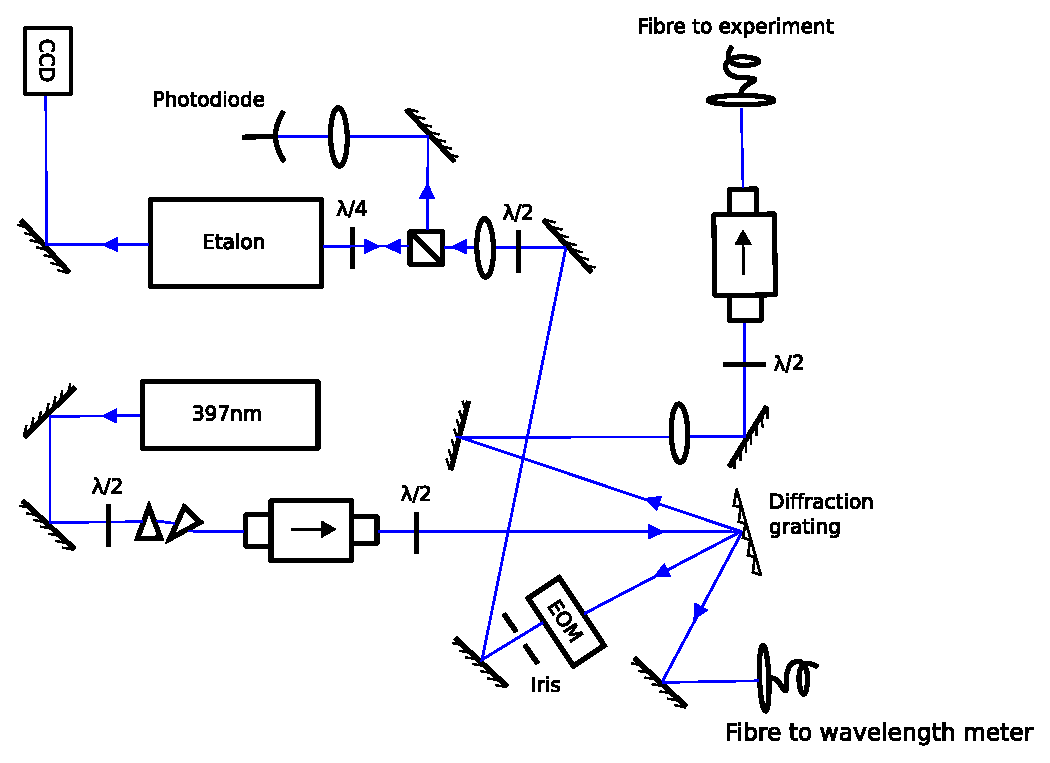
\includegraphics[width=13cm]{chapter4/397layout/397layout_v2}
%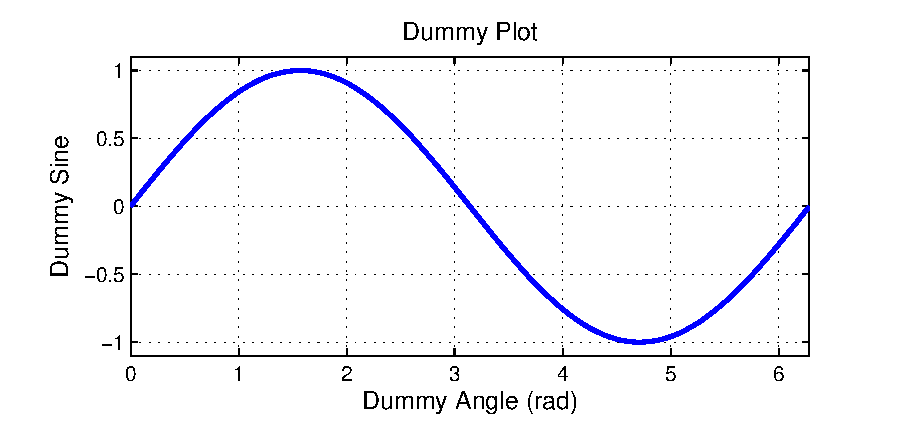
\includegraphics[width=5cm]{dummy}
\caption[397nm laser layout]{Layout of the 397nm laser system. Details in the text. Arrows on the beampaths show the direction of beam propagation. (Colour in electronic version)}
\label{fig:397layout}
\end{figure} 

\begin{figure}[h!t]
\begin{center}
$\begin{array}{c}
\mbox{\bf (a)} 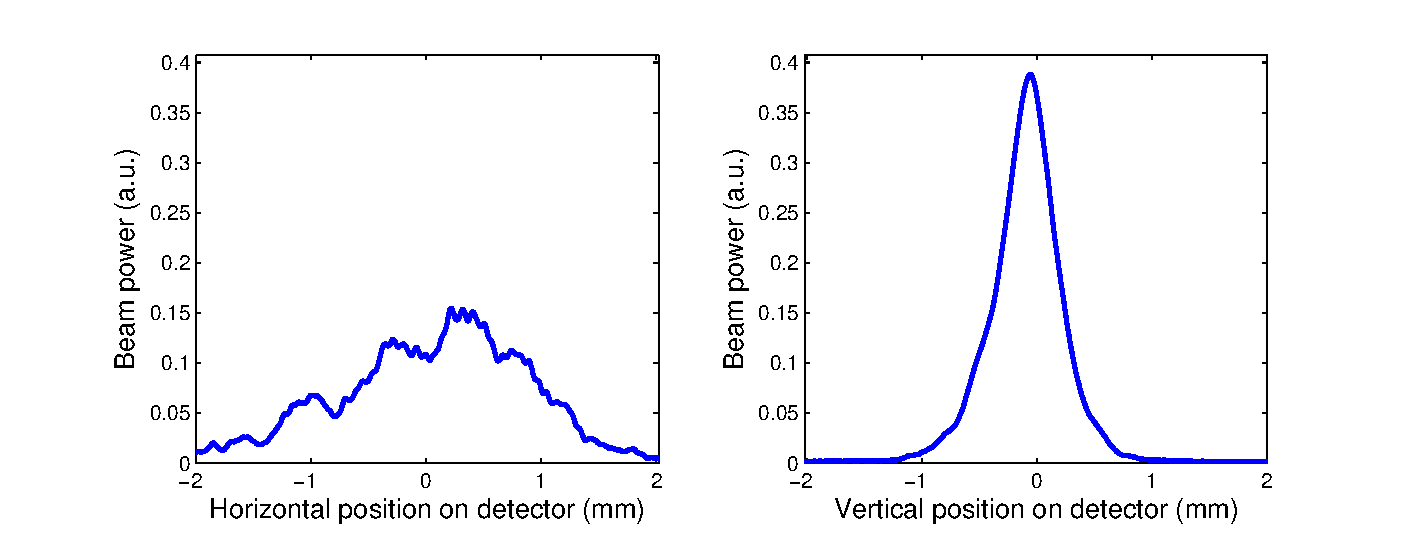
\includegraphics[width=13cm]{chapter4/beamprofile/397_laser_out}\\
\mbox{\bf (b)} 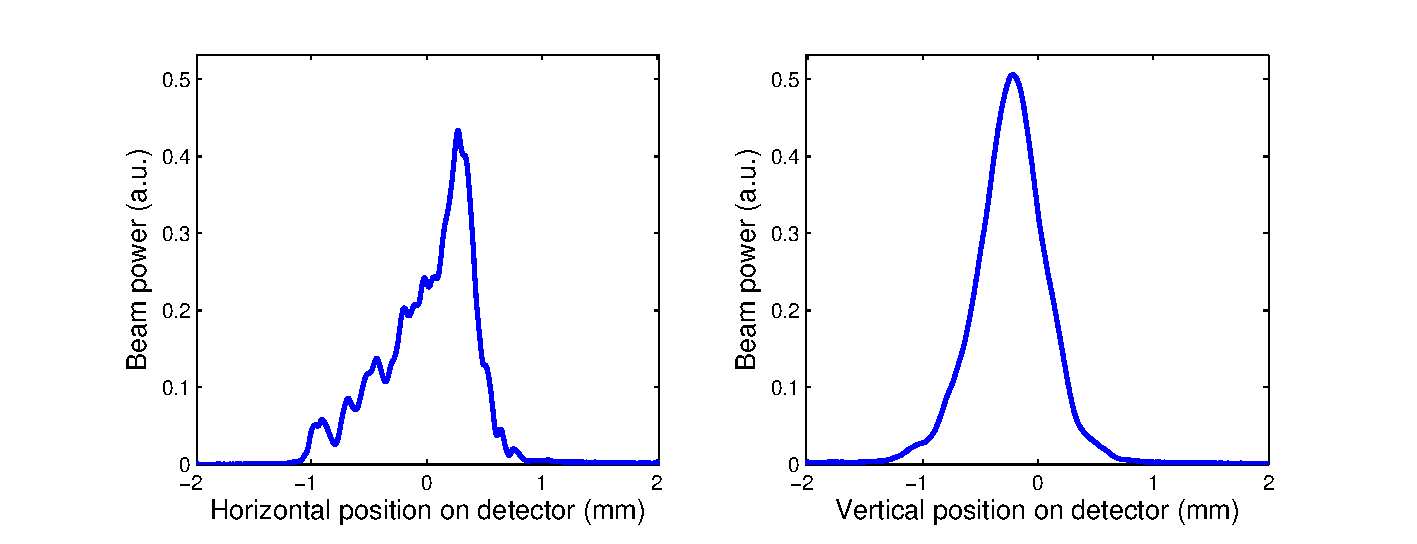
\includegraphics[width=13cm]{chapter4/beamprofile/397_after_prism_pair}\\
\mbox{\bf (c)} 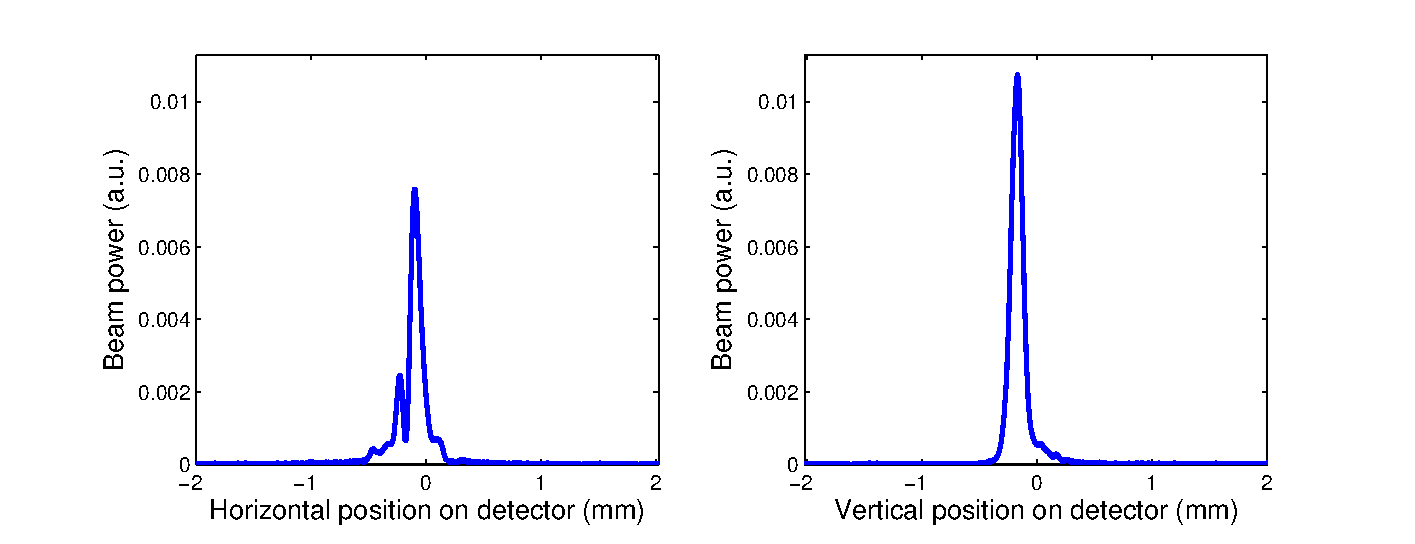
\includegraphics[width=13cm]{chapter4/beamprofile/397_before_fibre_in}\\
\end{array}$
\end{center}
\caption[Beam profiles of the 397nm laser]{Beam profiles of the 397nm laser, at different points in the optical path. a) the laser output, b) after an anamorphic prism pair, c) the ``experimental beam'' before its fibre input. Measurements were taken with a Thorlabs BP104-UV beam profiler. Laser intensities are in arbitrary units. The laser output has a large horizontal extension, which is reduced with the prism pair. The fibre input beam is small in order to maximise the fibre coupling.}
\label{fig:397beamprofile}
\end{figure}

The optical layout of the 397nm laser system is shown in Figure~\ref{fig:397layout}. The spatial profile of the output beam of this laser is highly non-Gaussian, see figure \ref{fig:397beamprofile}. The horizontal extent of the beam is quite large, and it has a ``halo'' area, that extends well beyond the detection area of the beam profiler used (the sensor area has 2\mm\, radius). An anamorphic prism pair makes the beam more circular, though with limited success. %This may be due to clipping of the extended beam on the prisms or that the beam is too far from being Gaussian.

A Toptica optical isolator  is used to reduce the back-reflection into the laser diode. The Thorlabs GR13-1204 diffraction grating (1200 grooves/\mm, blaze-wavelength of 400\nm) divides the beam into three beampaths. Order +1 is coupled into a multimode-mode fibre which leads to the wavemeter system, 0 is used for frequency stabilization and -1 provides the experimental beam.

\subsubsection{Frequency stabilisation of the 397nm laser}

Order 0 goes through a Leysop PM type EOM which modulates the beam at 85\MHz\, for the frequency locking system. The modulation voltage is supplied by the KILL module in the laser control box and is amplified by a Minicircuits RF amplifier. The beam then passes through an iris to clean the profile, a $\lambda/2$ plate to set the polarisation, and a 25 mm focusing lens. The transmitted beam after the NPL reference cavity is monitored by a CCD camera for diagnostic purposes. The reflected beam is picked off by the PBS cube (after twice passing through the $\lambda/4$ plate to rotate the polarisation by a total of $90\degree$) and directed onto a Hamamatsu C5331 avalanche photodiode. The photodiode signal is demodulated by the KILL module, and the output goes to the locking module of the Toptica laser control box. 

% This arrangement provides reliable PDH locking

It has to be noted that, while usually the TEM00 mode of the reference cavity is the most suitable for locking, in this case the TEM10 mode appeared to have better properties (larger capture range and better stability) so it was used instead. This is possibly due to the non-Gaussian spatial profile of the beam.

The control of the 397\nm\, laser frequency was similar to that for the 866\nm\, beam. One difference between the two is, however, that the control voltage to the 397\nm\, cavity's piezo controller was reduced with an 11:1 voltage divider, to allow finer control of the laser frequency, at the expense of scanning range. The calibration of the frequency adjustment, together with the used piezo driver base voltage, is shown in Table~\ref{tab:lasercalib}


\subsubsection{Experimental beam of the 397nm laser}

The experimental beam originally had only a focusing lens before coupling into the single-mode fibre which does not maintain polarisation (non-PM). However, because the fibre had a flat polished face, there was enough reflected power to deteriorate the laser diode performance, even with the optical isolator in place.  To eliminate this effect and improve stability, a second optical isolator was installed. The feedback effects stopped, but the optical isolator reduced the available laser power at the fibre output. Without the second optical isolator the maximum output power was approx. 200\uW; with the second optical isolator is in place this drops to 40\uW. Most of the experiments described in this thesis needed laser powers only $\sim$10-20\uW, but in the longer term several improvements are planned for the experimental beam. Using angle-polished fibres would eliminate the need for the second isolator since they reduce back-reflection and thus the optical feedback to the laser diode. A double-pass AOM would make possible fast switching of the beam, and also laser power stabilisation via an electronic feedback loop. 

\subsection{854nm repumping laser setup}
\label{subsec:854setup}


Early in the experiments to load an ion into the trap, the fluorescence signal had behaviour reminiscent of ``quantum jumps'' if the oven and photoionisation lasers were left turned on after capturing an ion (see Section~\ref{sec:ionload}). The fluorescence signal disappeared and reappeared in a timescale of a few seconds. 

The effect was due to shelving by the 389nm laser beam. It off-resonantly excites the ion into the \pth\, state, from where the ion can decay into the \dfh\, metastable state. While the ion is in the \dfh\, state, the Doppler cooling lasers cannot interact with it, which results in loss of fluorescence. During the time the ion is shelved and not cooled, it can also be heated up enough to leave the trap. 

There are two ways to eliminate this effect. The photoionisation lasers can be blocked immediately after ion capture. This method is used when loading a single ion. When blocking the photoionisation lasers is not possible (for example when trying to load multiple ions into the trap), a 854nm beam is used to repump from the \dfh\, to the \pth\, state, deshelving the ion.

The requirements for this beam are not very stringent in our experiment. The frequency stability necessary is much less than for the 866\nm\, and 397\nm\, beams. High power in the beam relaxes this requirement, as the power broadening makes it possible to interact off-resonantly with the ion even with significant ($\sim 100\MHz$) detuning. 

The 854\nm\, laser is also a Toptica DL100 diode grating stabilised in Littrow configuration. The layout of the system is shown in Figure~\ref{fig:854layout}. A Newport 53-004ZD02-035R diffraction grating splits the laser output into two beams, one for frequency diagnostics, one for the experiment. A double pass AOM is used for turning the beam on and off. A single-mode non-PM fibre is used to bring the experimental beam to the trap optical system.  The current coupling efficiency is $\sim20\%$ and the setup provides  $\sim 1\mW\,$ of power at the fibre output end. This power proved to be sufficient, though it might be possible to achieve higher output power by improving the coupling with an additional focusing lens before the fibre coupler.

\begin{figure}[h!t]
\centering
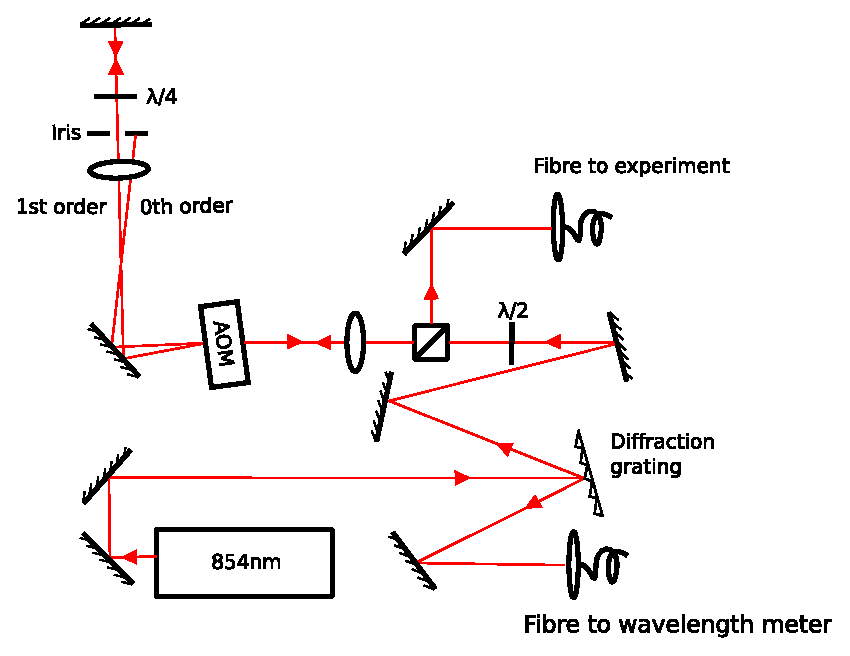
\includegraphics[width=13cm]{chapter4/854layout/854layout_v3}
%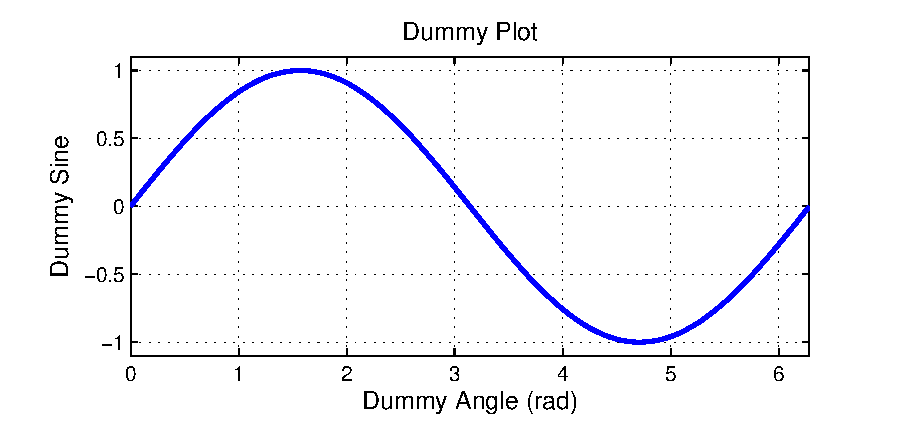
\includegraphics[width=5cm]{dummy}
\caption[854nm laser layout]{Layout of the 854nm laser system. Details in the text. Arrows on the beampaths show the direction of beam propagation. (Colour in electronic version)}
\label{fig:854layout}
\end{figure} 


\subsection{Laser diagnostics}

For coarse diagnostic of laser frequencies, a HighFinesse WS/7 wavelength meter was used. It is connected to a 8-to-1 fibre switcher, which allows us to monitor 8 different lasers at the same time.

A small portion of the laser light (10-100\uW) in each optical setup is coupled into a multimode fibre, and connected to one of the channels of the fibre switcher. The 8 channels of the switcher are sampled periodically, and the wavelength meter's control software displays measurement results.

The wavelength meter has a precision of 50\MHz\, in determining the laser frequencies. However, we observed a periodic fluctuation in the wavelength reading, see Figure~\ref{fig:wavemeterlong}. The fluctuation has amplitude approximately 40\MHz\, and period approximately 20 minutes. The long term stability is good.
As discussed in section \ref{sec:aircond}, this periodic change is probably due to the effect of the air conditioning system. The wavelength meter is located beneath one of the air ducts of this system, and probably the changing airflow interferes with the precision measurements. Moving the wavelength meter to a more suitable position is currently under way. 

\begin{figure}[t]
\centering
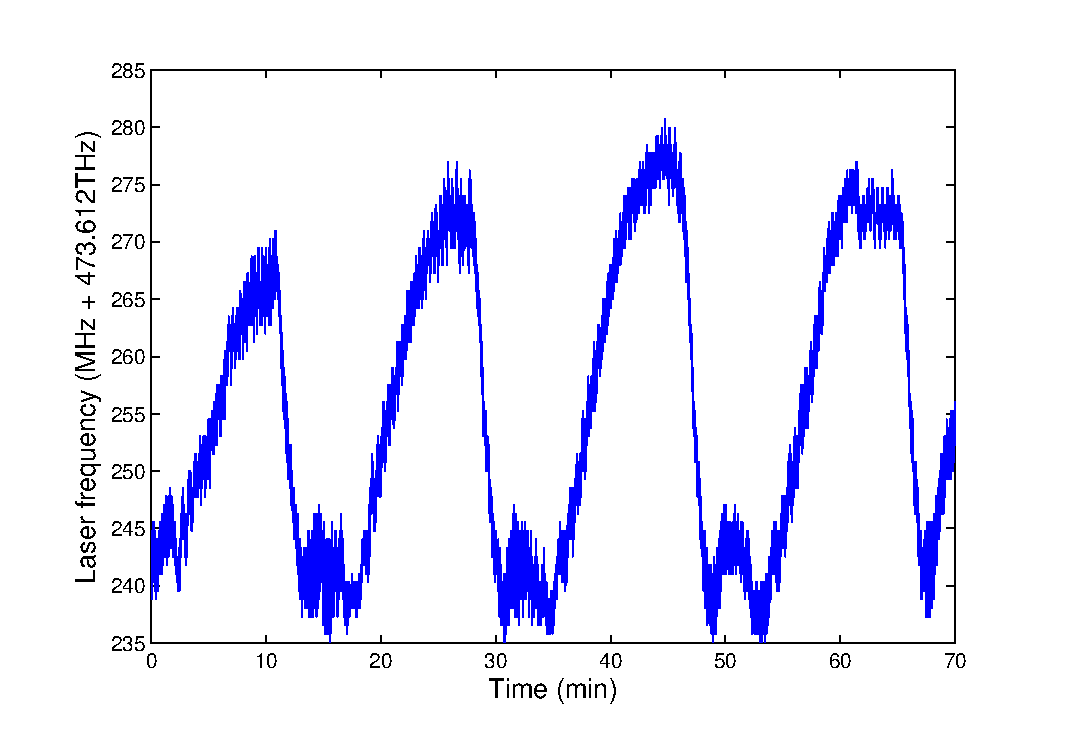
\includegraphics[width=10cm]{chapter4/wavemeter/HeNe_long}
\caption[Wavemeter long term diagnostics]{Frequency reading of a frequency stabilised HeNe laser (SIOS SL02/1) on the HighFinesse WS/7 wavelength meter. A section of a 6h logging period is shown. The laser has specified maximum excursion of $\pm 25$ MHz. A similar effect has been observed with the cavity-locked 866nm and 397nm lasers.}
\label{fig:wavemeterlong}
\end{figure} 

Because of this periodic change and the inadequate precision, we use the wavemeter reading for coarse adjustments and to monitor whether the laser locking mechanism is operating correctly or an unlocked laser is drifting too far from the set point. 

%There are plans to implement a more thorough laser diagnostics system, a prototype of which is already in use with the previous generation of our ion traps. The new system includes two spectrum analysers (one for the IR and one for the UV lasers) and more sophisticated software. The improved software allows us to monitor simultaneously the properties of up to 8 different lasers: wavelength, spectrum and locking signal on the same display. This prototype was created by D. Allcock \cite{Allcock2006}, and a copy of it will be built in the near future for the optical setup described here.

There are plans to implement a more thorough laser diagnostics system, a version of which is already in use with the previous generation of our ion traps. The new system includes two spectrum analysers (one for the IR and one for the UV lasers) and more sophisticated software. The improved software allows us to monitor simultaneously the properties of up to 8 different lasers: wavelength, spectrum and locking signal on the same display. This new system was created by D. Allcock \cite{Allcock2006} and a copy of it will be built for the optical setup described here in the near future.


\section{Trap optical setup}
\begin{figure}[h!t]
\centering
\includegraphics[width=13.5cm]{chapter4/trapoptics/trapoptics}
\caption[Optical setup at the trap]{Optical setup at the trap, with beam directions. The ``periscope'' denotes the part of the optical setup where the joint 423nm and 397nm vertical beams leave the plane of the other beams, and are guided through the viewport on the upper part of the vacuum chamber. Thus the beam which appears to be directed towards the imaging actually system passes beneath the main imaging lens. \cversion}
\label{trapoptical}
\end{figure} 

\begin{figure}[h!t]
\centering
\includegraphics[width=11cm]{chapter4/trapoptics/traplaserdir2}
\caption[Beam directions at the trap]{Schematic of the beam directions at the ion trap. The beam wavelengths are noted, together with the angles between the beams. (Colour in electronic version.)}
\label{beamdirections}
\end{figure} 


\subsection{Photoionising lasers}
\label{subsec:photionlayout}

The photoionising lasers (423nm and 389nm) are shared between the experiments in two labs. The laser sources are physically in another lab, the beams are superimposed on a PBS cube and coupled into a Nufern S405 single-mode fibre. At the fibre output originally both wavelengths were focused into the trap by the same lens. However, because of chromatic aberration, the two beams have a focal length difference of about 3 mm, which is comparable to the Rayleigh ranges of the beams.

For better focusing, the beams were separated into two beam paths. This could be done using a $\lambda/2$  waveplate and a PBS cube after the fibre output since the beams have orthogonal polarisation due to the way they are combined before the fibre. Better than 97\% of each beam power was in the right beam path. The 423\nm\, beam enters the vacuum chamber from a viewport on the top, the 389\nm\, beam through a side window. This allowed good focusing for both beams, which reduced scattered light, and smaller beam powers were sufficient to achieve the same loading rate.

Ideally, the 423\nm\, laser beam should be perpendicular to the atomic beam coming from the Ca oven, to minimise Doppler broadening. This would allow us to perform isotope-selective photoionisation, since the atomic excitation frequencies are different for the different \CaI{} isotopes. In our case, however, the placement of the Ca oven and the input ports put constraints on the angle between the atomic beam and the laser beam. In practice, this angle for  the natural abundance \CaI{} oven is $\sim 70\degree$. Because of its position, the angle between the oven containing $^{43}$Ca enriched sample and the laser beam is even smaller, $\sim 50\degree$ (see Figure~\ref{fig:vacuum} and \ref{fig:calciumoven}). The effect of these angles is discussed in Section~\ref{sec:atomfluo}, describing the experiments observing neutral atom fluorescence in our trap.


\subsection{Doppler cooling lasers}
\label{subsec:dopplertrapsetup}

Fibres were used for both the 397nm and 866nm laser beams to bring them to the trap. Originally there was a single 397nm beampath, which was focused down to the trap by a short focal length (100mm) lens. This lens was tilted with an angle of approx 14\degree\, such that it creates an elongated instead of a tight circular focus. The beam has waist $w_{0,horiz} = 87\mu$m in the horizontal direction and $w_{0,vert} = 25\mu$m in the vertical direction. The advantage of this arrangement is that while avoiding scattered light if the beam hits the RF electrodes in the vertical direction, there is still significant power in the beam along the trap axis in the horizontal direction. This allows us to move the ion a significant distance (approximately $\pm$ 50$\mu$m) along the trap axis, and still be able to cool it and observe a good photon scattering rate. The 866nm beam is superimposed on the 397nm light with a near-UV mirror, which reflects the 397nm beam and transmits infrared wavelengths. 

Early in the building of the optical setup a need for careful control of the beam polarisation was observed. The background scattered light had a significant polarisation dependence. Originally a $\lambda/2$ waveplate was used to minimise the background scatter by rotating the polarisation to be horizontal. This arrangement needed constant checking and tweaking. Subsequently, better performance was achieved by inserting a PBS cube into the beampath.

The transmitted beam of the PBS cube was used as the main experimental beam, the reflected beam was redirected and continued with the 423nm beam on the PBS cube already used to separate the two photoionisation beams. By use of appropriate lenses, it is possible to focus this secondary 397nm beam (or ``vertical'' beam)  onto the same place in the trap as the 423nm beam. 

While the horizontal beam has the whole 100\um\, spacing between the RF rails to propagate through, the vertical beam has a reduced available cross-section, due to the angle at which it arrives at the trap. Also, due to the direction of the vertical beam, scattered light is more likely to get into the imaging system than in the case of the horizontal beam.  We observed more than one order of magnitude higher background scatter counts on the PMT from the vertical beam than from the horizontal beam. Because of this  problem, the vertical beam is only used in experiments when it cannot be avoided. Normally, only the horizontal 397\nm\, beam is present.


\section{Polarisation and power stability}
\label{sec:beamstability}

Many experiments with trapped ions require good polarisation and power stability. The stability of the 397nm and 866nm beams were measured at their respective fibre outputs. For each beam, two photodiodes were positioned so to measure the transmitted and reflected beams of a PBS cube after the fibre output. 

The transmitted and reflected powers ($I_T$ and $I_R$, respectively) were recorded for several hours. The polarisation angle is calculated from:
\begin{equation}
\theta = \arccos\left(\sqrt{\frac{I_T}{I_T + I_R}}\right)
\end{equation}

\begin{figure}[h!t]
\begin{center}
$\begin{array}{c}
\mbox{\bf (a)} 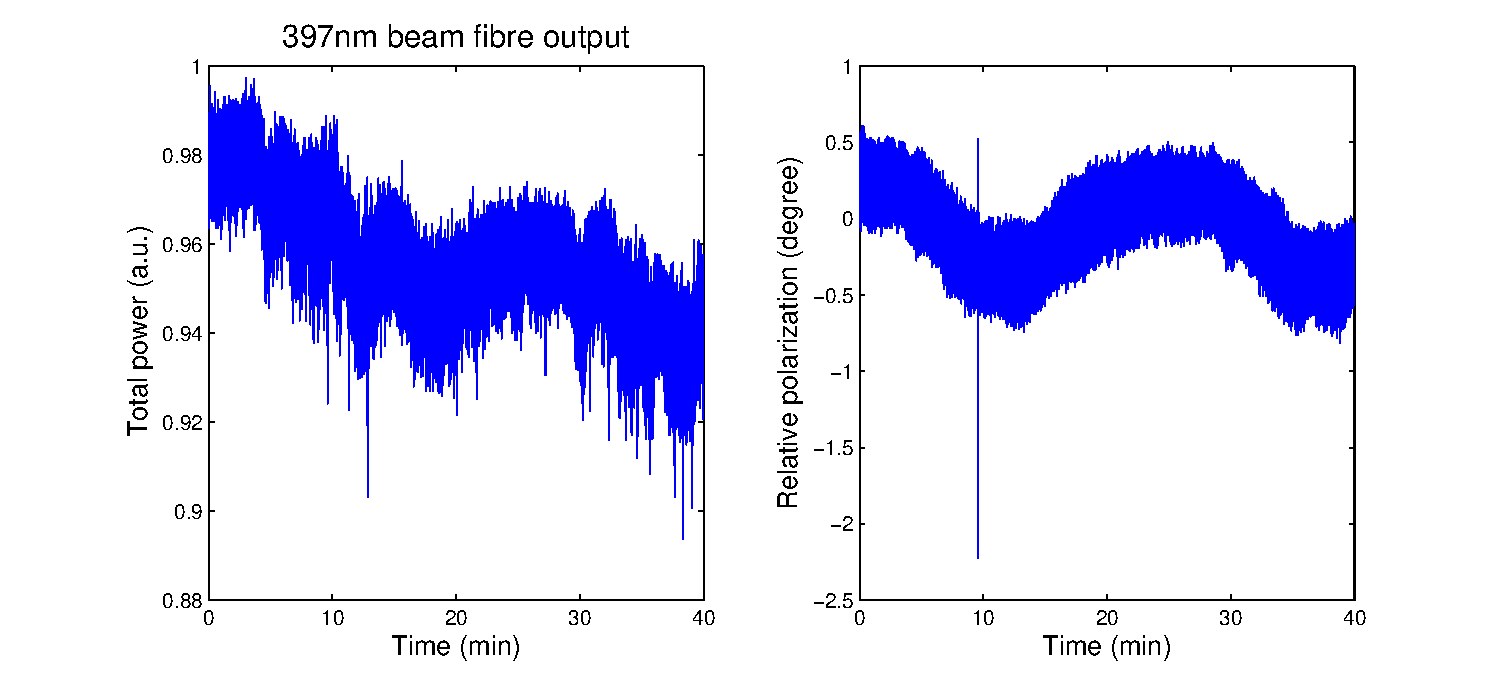
\includegraphics[width=14cm]{chapter4/polarisation/397pol}\\
\mbox{\bf (b)} 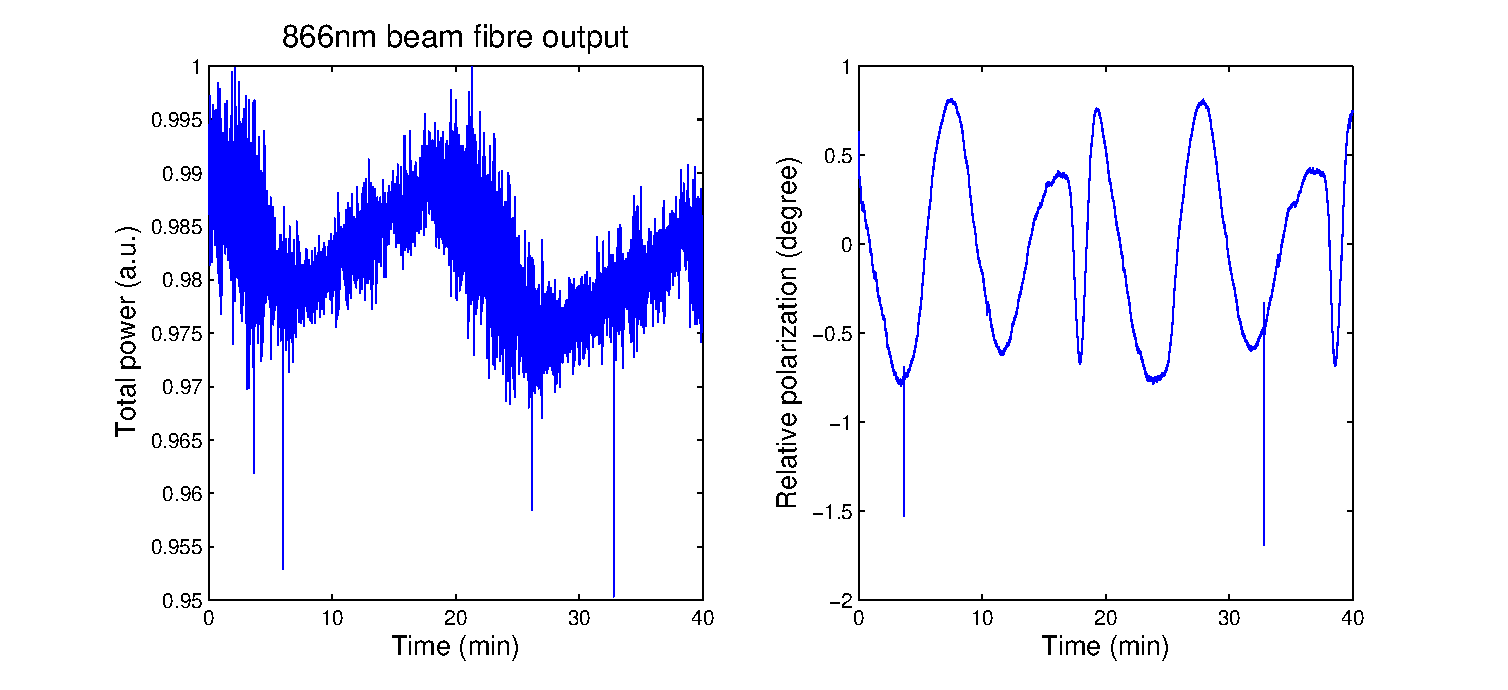
\includegraphics[width=14cm]{chapter4/polarisation/866pol}\\
\end{array}$
\end{center}
\caption[866nm and 397nm fibre output polarisation and intensity]{Fibre output polarisation and intensity for a) 397nm beam (non-PM fibre), b) 866nm beam (PM fibre). The PM fibre has better defined polarisation on seconds to minute timescales. Both fibres exhibit an approx. 20 minutes periodicity in polarisation (more obvious on longer recorded sequences, not shown here). The 866nm beam also shows periodicity in intensity, while in the 397nm beam it is hidden by the intensity drift. The ``dropouts'' are due to measuring photodiodes.}
\label{fig:fibreoutputs}
\end{figure}


Figure~\ref{fig:fibreoutputs} shows the total beam intensity ($I = I_T + I_R$) and the calculated polarisation angle $\theta$, as a function of time. It can be seen that both the powers and the polarisation, for both beams, have periodic structure, with an approx. 21 minutes period. This periodicity is correlated with the air conditioning system (see Section~\ref{sec:aircond}). 

The 866\nm\, beam has better defined polarisation on the short timescale (seconds), while the 397\nm\, beam has a short term variation of $\pm 0.25\degree$. On the several minutes timescale, the polarisation variation of the 866\nm\, is approximately $\pm 0.75\degree$, while the 397\nm\, beam has variations in the order of $\pm 0.5\degree$. 

One major difference between the two fibres is their stability against mechanical disturbances. The PM fibre of the 866nm beam keeps its polarisation if it is set up correctly, while the output polarisation of the non-PM fibre of the 397nm beam changes completely if it is touched. In the test experiment care was taken not to disturb the fibre, to be able to observe the additional (not ``accidental'') effects on polarisation.

The polarization stability of the non-PM fibre is somewhat improved by introducing a low level of stress to the fibre, by e.g. bending a section of it with a few cm radius. This arrangement makes the fibre birefringent which improves the polarisation stability along the fast axis. It also creates large bending losses if the bending radius is small. In our experiments the radius was large enough ($\sim$5-10\cm) not to introduce significant bending loss. Fortunately, the experiments described in this thesis are of a pilot nature and variations of polarisation of the order of a degree or so are of no significance.


Similarly, the periodic change of the fibre output power may also pose problems to more sophisticated experiments, in our case, however, this change was not significant. If needed, improved power stability can be achieved by a feedback loop with an AOM on the fibre input side. 



\section{Imaging system}

An outline of the imaging system is shown in Figure~\ref{fig:imagingsystem}. The vacuum chamber's largest viewport was chosen to be the detection route for the ion fluorescence signal. Its design allows a large imaging lens to be brought close to the viewport, thus increasing the solid angle in which the signal can be collected. 

\begin{figure}[h!t]
\centering
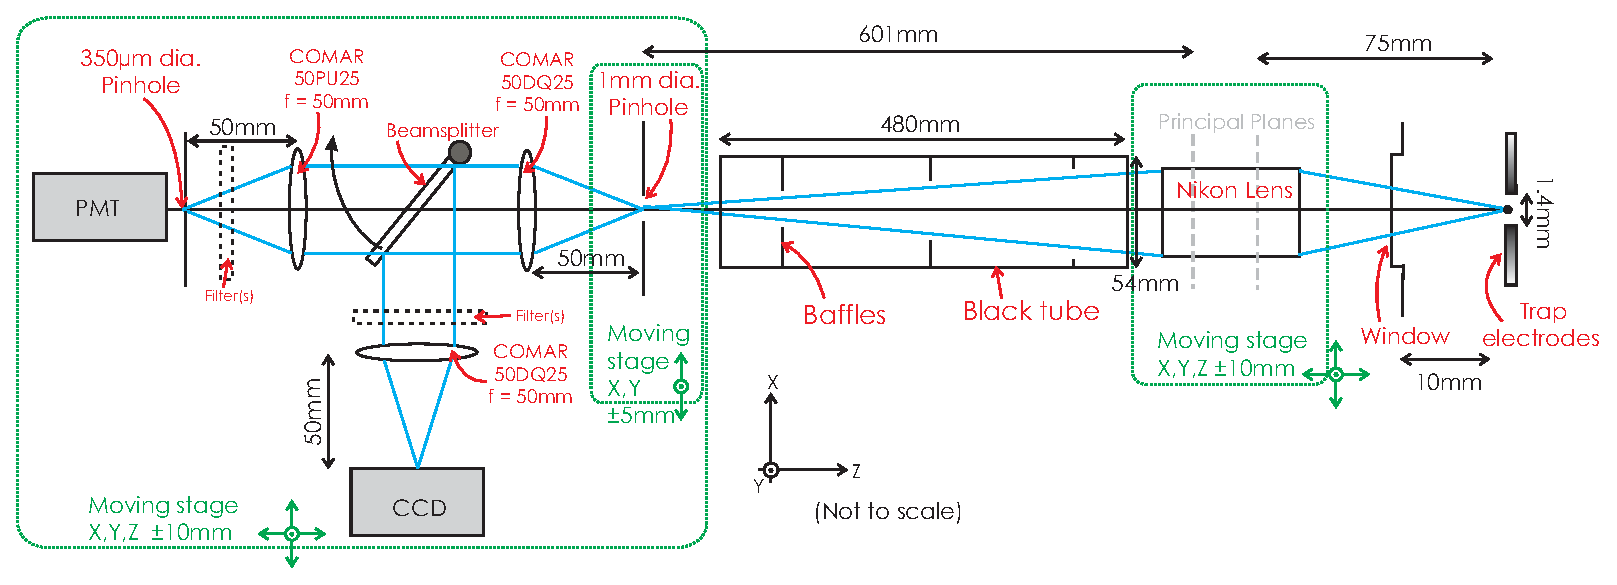
\includegraphics[angle=90,width=7.1cm]{chapter4/imaging/systplan}
\caption[Imaging system]{Schematic layout of the imaging system, from A. Myerson \cite{Myerson2007}}
\label{fig:imagingsystem}
\end{figure} 


A Nikon ED PLAN 1.5X wide aperture composite lens collects the light from the ion, with numerical aperture of $\sin\Theta\approx0.29$, which corresponds to a collection efficiency of $0.021$. The Nikon lens images the ion with a magnification of 8 onto a pinhole of 1\mm\, diameter. The pinhole is used to exclude light scatter from the trap electrodes. The light is re-imaged onto a photo-multiplier tube (PMT) and an image-intensified CCD camera (EEV Super Photon ICAM2-07-06E) using two lenses (Comar 50DQ25, $f = 50\mm$). A beam-splitter is used to divide the light into two beam paths for the PMT and the CCD. When visual information about the ion is not needed, the beam-splitter can be moved out of the beam path, to maximise the fluorescence signal on the PMT.

A pair of interference filters are placed in front of the PMT to transmit only around 397\nm. They are mostly aimed at reducing background light from the photoinisation beams at 389\nm\, and 423\nm.  

A second, smaller pinhole of 350\um\, diameter is placed in front of the PMT, further reducing the background scattered light, while transmitting the fluorescence from the ion. The PMT is connected to the measurement control computer, which processes its output.

Table~\ref{tab:efficiency} contains the calculation of the estimated detection efficiency, based on the parameters of the optical elements, which gives $\eta = 0.16(3)\%$. The error is calculated assuming a 10\% error on the collection efficiency and 5\% error on all other parameters. For the neutral atom fluorescence experiments (see Chapter~\ref{chapter:firstobs}) the interference filters were removed, thus the estimated detection efficiency was $\eta = 0.19(3)\%$.

More details of the imaging system are given in Appendix C of \cite{Myerson2007}.

\begin{table}[ht]
 \begin{center}
% use packages: array
\begin{tabular}{lr}
\hline
Collection efficiency			& 0.021 \\
Output window $T$ 				& 0.92 \\ 
Nikon lens $T$				 	& 0.73 \\ 
$2\times$ Comar lens $T$		& 0.85 \\ 
Interference filters $T$		& 0.86 \\
PMT quantum efficiency at 397\nm & 0.16\\
\hline
Overall detection efficiency & 0.16(3)\% \\
\hline
\end{tabular}
\end{center}
\caption{Summary of the calculation of the expected detection efficiency of the photon collection system.}
\label{tab:efficiency}
\end{table}



\section{Electronics}

\subsection{Control computer}

The experimental apparatus is controlled by a central computer. Two digital-analog input/output cards (DAC) (PCI DAS-1200 and PCL-727 models) are used to interface the various items of equipment (see Figure~\ref{fig:controlcomp}). 

The experimental control program running on this computer uses a time-to-amplitude converter (TAC) to read photon counts from the photomultiplier tube (PMT). The sync signal of the RF voltage source is also connected to the TAC, to provide information about correlation between the RF-phase and photon arrival times. This correlation information was used for ion motion diagnostics, see Section~\ref{sec:micromotioncomp}.

The PCI DAS-1200 card is used for most of the experimental control. One of the DAC analog input channels records the ion gauge current for pressure measurement and another channel logs the photodiode current in some experiments to measure laser intensities. 

A digital output channel triggers a shutter to block and unblock the photoionisation beams at their fibre output, and another digital channel controls the AOM driver of the 866nm laser setup. Analog output channels control the wavelength of the cavity-locked 397nm and 866nm by piezo-control of the cavity length. The calibration of these channels is shown in Table~\ref{tab:lasercalib}.

The PCL-727 card provided extra analog and digital outputs when needed.


\begin{figure}[h!t]
\centering
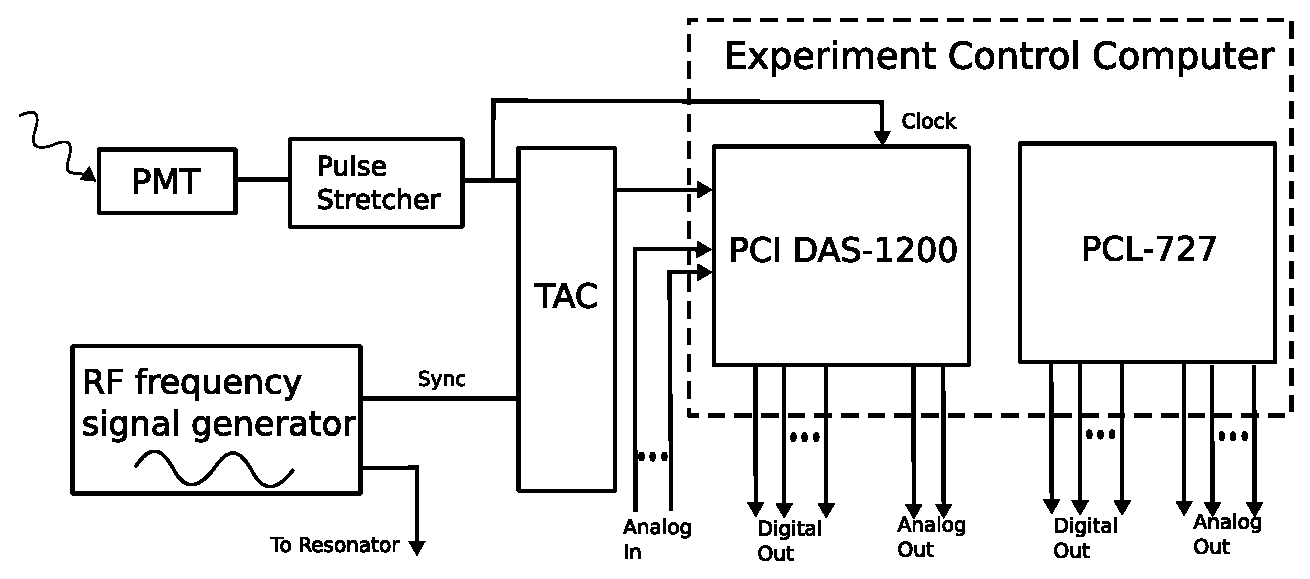
\includegraphics[width=13cm]{chapter4/computer/computer}
\caption[Experiment control computer connections]{The connection layout of the experiment control computer. The wiring information of the PCI DAS-1200 and PCL-727 cards and the connected input and output channels are in the text.}
\label{fig:controlcomp}
\end{figure} 



\subsection{DC electrodes and secondary control computer}
\label{sec:dcelectrodecontrol}

In the early experiments the voltages for DC electrodes were provided by TTi stabilised power supplies. However, this only allowed restricted setting of the electrodes. Because of the limited number of power supplies, many of the DC electrodes had to be set to the same voltage. For the first attempt to trap ions this was sufficient. As soon as compensation of stray electric fields was necessary for more sophisticated experiments, the number of power supplies and their control became a limiting factor.

Ultimately the setup was changed such that the DC electrodes were controlled by computer via a Measurement Computing DAC6703 16-channel D/A converter card. 14 channels were used to set voltages in the $\pm 10\V$ range separately for all 14 DC electrodes. This allows complete compensation of the electric field. The computer control is also capable of outputting voltage waveforms to the electrodes to move ions in the trap.

The outputs of the DAC card are distributed by a breakout box with BNC connectors. This is connected to a second, specially designed box to package voltages from different sources into a D-type cable, which delivers them to the vacuum feedthrough that is connected to the ion trap chip carrier inside the vacuum system. The BNC cables provide better shielding against electromagnetic noise than the D-type cable.

To reduce the electromagnetic noise, a filter box was inserted between the vacuum feedthrough and the D-type cable. The filter box contained a separate RC circuit as a low pass filter (R=1.8\kOhm, C=0.1\uF, time constant $\tau = 0.18\us$) for each voltage supply line to the DC electrodes, 14 filters altogether.  A detailed investigation of the issue of electromagnetic noise and its effect on the ion is discussed in Section~\ref{sec:filternoise}.

The control computer for the electrodes is separate from the measurement computer. The voltages were set by a Matlab graphical interface program developed for this task, running on Windows or Linux, depending on the experiment conducted, because of certain limitations of both systems. More about the specific control program will follow in the section describing the various experiments.

In addition to controlling the DC electrodes, this secondary control computer is also used to capture images of the ions, by connecting to the CCD camera of the imaging system. 




\subsection{Helical resonator}
\label{sec:helicalresonator}
To amplify the radio-frequency voltages applied to the RF electrodes in the ion trap, we use a helical resonator \cite{McAlpine1959}. It was built by J. P. Home \cite{Home2005}. The resonance frequency was measured to be 27.25MHz, and the Q-factor of the resonator was determined to be approximately 20. This, however, can be only checked before connecting the resonator to the electrodes, which means the actual Q-factor (and hence the exact voltages applied to the RF electrodes) is unknown.  The Q-factor can later be deduced by comparing observed radial trap frequencies with calculation from the electrode geometry. The experiment is described in Section~\ref{sec:ticleexperiment} and the results are consistent with the predictions.

The output of the helical resonator is connected to the RF rails through a vacuum feedthrough on the top of the vacuum chamber (see Figure~\ref{fig:vacuum}).  The connections had to be carefully made to minimise the losses and deliver as much power as possible to the RF rails.


\section{Air conditioning}
\label{sec:aircond}

Air conditioning is a new feature of the refurbished labs. It provides greater temperature stability, which is very helpful for the optical setup. However it is not perfect. To check how efficiently the air conditioning system stabilises the temperature, a long term (25 days) temperature logging was conducted in the lab, with two temperature sensors (see Figure~\ref{fig:airconditioning}). The lack of a reheating module in the air conditioning system means there is a 0.5\degree\, temperature swing, on the time scale of approximately 20 minutes. Beside the short time scale temperature change, there is also a daily variation. 

The effect of this temperature change is clearly visible on the precision elements of the optical setup, as already noted. The laser fibres are the most affected; the polarisation and intensity of the output beams change with similar periodicity to the temperature. There are various possibilities for the cause of this correlation. The way the fibres are routed close to the ceiling between the optical and experimental table brings them close to the air outputs of the air conditioning system. Changes of airflow during the air conditioning cycle or the temperature change may cause mechanical stress in the fibres. This might be reduced by using thicker protective tubing for the fibres, but this is yet to be tested.

The effect of the air conditioning on the wavemeter is harder to eliminate. Fortunately most of the time precision wavemeter readings are not essential for the experiment. The wavemeter serves as a crude and quick diagnostic for laser frequency jumps or drifts. Precision frequency measurements are done using the atomic transitions and fluorescence.

\begin{figure}[h!t]
\centering
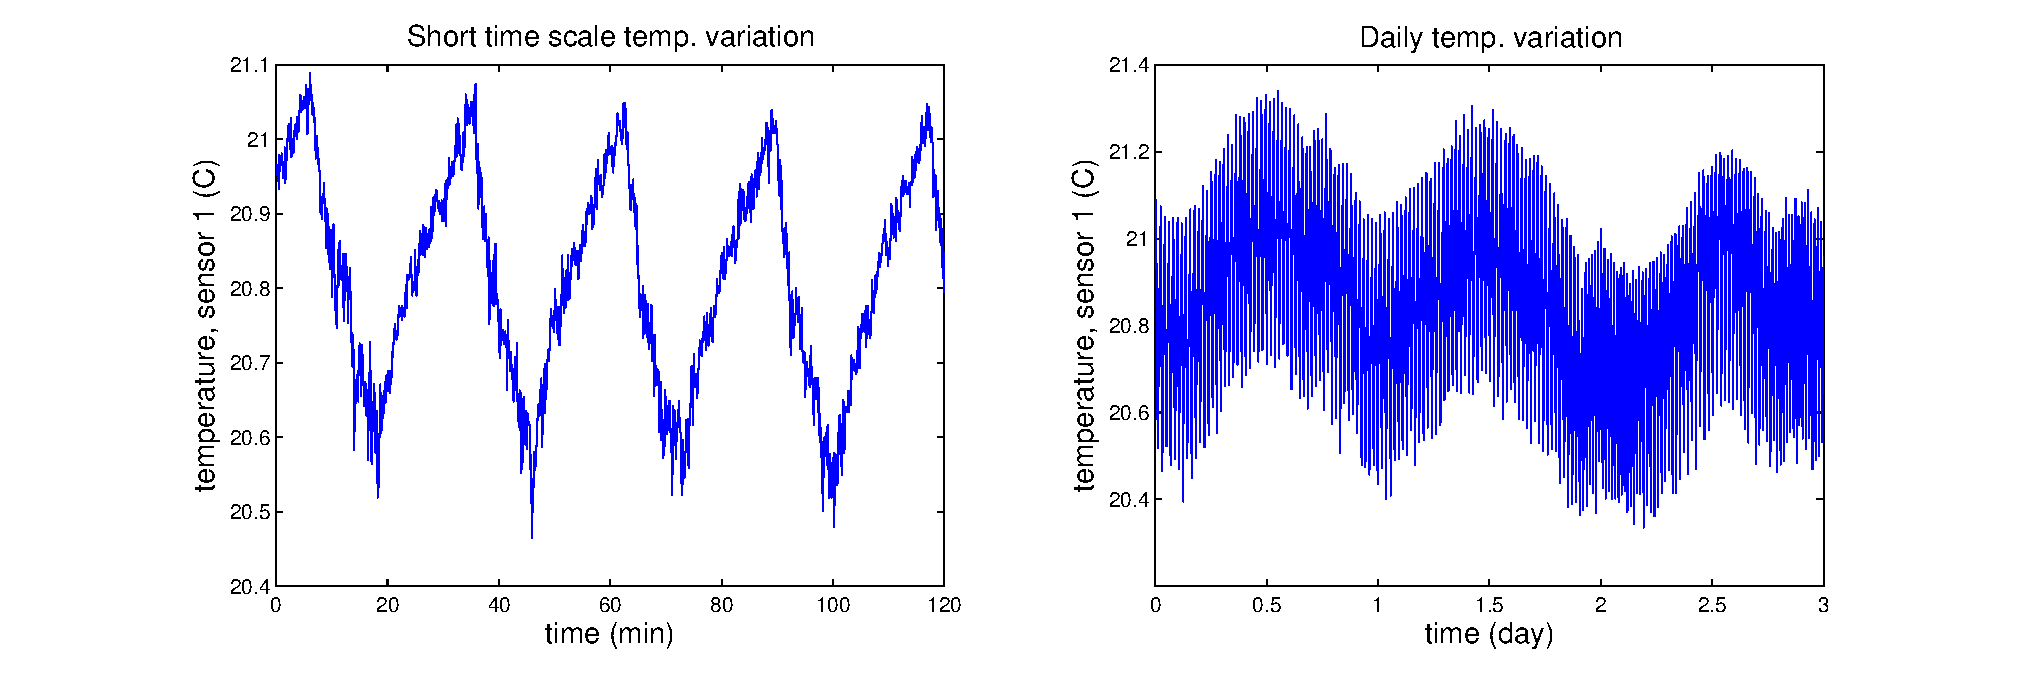
\includegraphics[width=14.5cm]{chapter4/aircond/aircondsmall}
\caption[Lab temperature variations]{Temperature variations of the lab measured by a thermocouple placed on the shelf containing the wavelength measurement hardware. The periodicity is in step with the the air conditioning system's on/off cycles. Both short time scale and daily variations are present.}
\label{fig:airconditioning}
\end{figure} 


